\documentclass[spanish]{beamer}
%

% esto me setea la variable pdf dependiendo del valor de \pdfoutput, que es >0
% sólo cuando estoy usando pdflatex para compilar el documento
\newif\ifpdf
\ifnum\pdfoutput<0
\pdffalse\fi
\ifnum\pdfoutput=0
\pdffalse\fi
\ifnum\pdfoutput>0
\pdftrue\fi

%\makeatletter
%\def\markboth#1#2{\def\leftmark{\@IEEEcompsoconly{\sffamily}\MakeUppercase{\protect#1}}%
%\def\rightmark{\@IEEEcompsoconly{\sffamily}\MakeUppercase{\protect#2}}}
%\makeatother

%
% ===
% === I18n / L10n
% ===
%
% babel me da separación de sílabas para palabras en el idioma que le paso como
%       argumento opcional. <-- Éste hay que pasarlo en \documentclass
\usepackage[spanish]{babel}
%
% inputenc define la codificación de caracteres del código fuente, acá utf8.
\usepackage[utf8]{inputenc}
%
% ===
% === Gráficos
% ===
% 
% pst-pdf me permite usar PSTricks con pdflatex. Necesito cargarlo sólo si está
%         definida la variable pdf, por eso está entre \ifpdf ... \fi
%\ifpdf\usepackage{pst-pdf}\fi
%
% color me permite usar colores en el documento.
\usepackage{color}
%
% graphicx me da el comando \includegraphics para insertar imágenes (?)
\usepackage{graphicx}
%
% pstricks es un conjunto de macros basadas en PostScript para TeX, en
%          castellano, me da un entorno pstricks y comandos que uso dentro de
%          éste, que me sirven para dibujar figuras/diagramas/etc de manera
%          relativamente simple.
%\usepackage{pstricks}
%
% pst-circ me da macros para pstricks que me dibujan elementos de circuitos
%\usepackage{pst-circ}
%
% 
%\usepackage{pst-plot}		%Para dibujar una curva a partir de un archivo
%\usepackage{pst-2dplot}		%Para plotear. entorno pstaxes
%
% ===
% === Verbatims
% ===
%
% verbatim es una reimplementación de los entornos verbatim[*]
%          provee el comando \verbatiminput{archivo} y el entorno comment, que
%          hace que LaTeX ignore directamente todo lo que está adentro
%\usepackage{verbatim}
%
% moreverb implementa el entorno verbatimtab indentando los tabs que encuentre,
%          y también el entorno listing, que pone números de línea al verbatim.
%          Para cambiar el ancho de la tabulacion, uso
%          \renewcommand\verbatimtabsize{<ancho del tab>\relax}
%          También define el entorno boxedverbatim.
%\usepackage{moreverb}
%
% listings me da el entorno lstlisting con resaltado de sintaxis.
%          Para setear el lenguaje del código, hago \lstset{language=<lang>}
%\usepackage{listings}
%
% url es un verbatim para escribir URL's que permite linebreaks dentro de ésta.
%     para usarlo, \url{<URL>}
\usepackage{url}
%
% ===
% === Estilos, etc..
% ===
%
% ulem me da comandos para subrayar y tachar. Por defecto, modifica el
%      comportamiento del comando \emph, haciendo que subraye en vez de poner
%      el texto en cursiva. Este comportamiento se revierte con el arg opcional
%      normalem.
\usepackage[normalem]{ulem}
%
%
%\usepackage{mdwlist}		%Para listas mas compactas
%\usepackage{textcomp}		%Para algunos símbolos
%\usepackage{colortbl}		%Para celdas de colores en tablas
%\usepackage{fancyhdr}		%Para encabezados/pie
%\usepackage{bbold}		%Fuente bb para modo math: \mathbb{R} = reales
%\usepackage{dsfont}		%Fuente ds para modo math: \mathds{R} = reales
\usepackage{multirow}		%Para "combinar" celdas en tablas
%\usepackage{float}		%Para cuadros, figuras, etc copadas
%\usepackage{fancybox}		%Para recuardos de texto con bordes "fancy"
%\usepackage{dingbat}		%Para dingbats
%%\usepackage{marginal}		%Para notas al margen que no puedo hacer andar
\usepackage{amsmath}		%Para enornos matemáticos mas flexibles
%\usepackage{varwidth}		%varwidth es un minipage que se ajusta al ancho mínimo
\usepackage{pslatex}            % setea fuentes Times, Helvetica y Courier ``angosta''
\usepackage{latexsym}



%Estilos de texto
\newcommand{\resalt}{\colorbox{green}}	%Resaltado - Fondo verde
\newcommand{\sfbf}{\bfseries\textsf}	%Slanted + Bold
\newcommand{\eng}{\textit}			%Palabra en inglés - Itálica
\newcommand{\mean}{\textsl}			%Significado de una sigla - Slanted
\newcommand{\defin}{\textbf}			%Definición - Negrita
\newcommand{\R}{\mathds}			%Para escribir R de Reales, N de Nat
\newcommand{\N}{\mathbf}			%Para escribir R de Reales, N de Nat
\newcommand{\lil}[1]{\footnotesize #1}
\newcommand{\mono}[1]{{\tt #1}}         % Monoespaciado


%Símbolos
\newcommand{\y}{\wedge}			%Y (Lógica)
\newcommand{\ve}{\vee}			%O (Lógica)
\newcommand{\ent}{\supset}		%Entonces (Lógica)
\newcommand{\dimp}{\leftrightarrow}	%Doble implicativo, equivalencia (Lógica)
\newcommand{\sii}{\leftrightarrow}	%Si y sólo si (Lógica)
\newcommand{\equi}{\equiv}		%Equivalencia (Lógica)
\newcommand{\portanto}{\vdash}	%Por lo tanto (Lógica)
\newcommand{\por}{\cdot}		%Producto punto

%Configuraciones del documento
%\selectlanguage{spanish}		%Elijo idioma español

%Tweaks
%\setlength{\parindent}{0mm}		%Sangría de 1a. línea
%\setlength{\hoffset}{-5.4mm}		%
%\setlength{\voffset}{-5.4mm}		%
%\setlength{\topmargin}{0mm}		%
%\setlength{\oddsidemargin}{5mm}	%
%\setlength{\evensidemargin}{5mm}	%
%\setlength{\marginparsep}{5mm}	%
%\setlength{\headheight}{12.5mm}	%
%\setlength{\headsep}{2.5mm}		%
%\setlength{\footskip}{10mm}		%
%\setlength{\textwidth}{15cm}		%
%\setlength{\textheight}{232mm}	%
%\setlength{\fboxrule}{.1pt}
%\setlength{\parskip}{.5\baselineskip}
%Colores
\definecolor{negro}	{cmyk}{0,0,0,1}
\definecolor{marron}	{cmyk}{0,.5,1,.41}
\definecolor{rojo}	{cmyk}{0,1,1,0}
\definecolor{naranja}	{cmyk}{0,.35,1,0}
\definecolor{amarillo}	{cmyk}{0,0,1,0}
\definecolor{verde}	{cmyk}{1,0,1,0}
\definecolor{azul}	{cmyk}{1,1,0,0}
\definecolor{violeta}	{cmyk}{.45,1,0,0}
\definecolor{gris}	{cmyk}{0,0,0,.5}
\definecolor{blanco}	{cmyk}{0,0,0,0}
\definecolor{dorado}	{cmyk}{0,.16,1,0}
\definecolor{plateado}	{cmyk}{0,0,0,.25}

%Comandos personalizados
\newcommand{\T}{\textrm}%Para escribir texto común cuando en modo math

% Remarca un ``texto insertado'' en rojo. Necesita el backage color.
\newenvironment{ins}{\color{red}$>$}{$<$}
\newcommand{\iins}[1]{{\color{red}$>$#1$<$}}

% Tacha un texto. Depende del package ulem.
\newcommand{\tachar}{\sout}

% Tacha doble
\newcommand{\Tachar}[1]{\sout{\sout{#1}}}

%\newcommand{\}

%\begin{pspicture}
%\def\tierra(#1){%Para dibujar el símbolo de tierra en el entorno PSTricks
%	\rput(#1){
%		\psdot(0,0)
%		\psline(0,0)(0,-0.45)
%		\psline(-0.5,-0.45)(0.5,-0.45)
%		\psline(-0.35,-0.6)(0.35,-0.6)
%		\psline(-0.2,-0.75)(0.2,-0.75)
%	}%
%}
%\end{pspicture}

%\newcommand{\codigo}[2]{%Para generar un recuadro con código
%	%\setlength{\hrulewidth}{0.1pt}
%	\begin{flushleft}
%	\underline{#1}
%	\begin{tabular}{@{\quad}|l}
%		\begin{minipage}{.85\textwidth}\smallskip{#2}
%	\end{minipage}\end{tabular}\end{flushleft}%
%}

%\newcommand{\filecodigo}[1]{%Insertar código verbatim desde un archivo
%\codigo{#1}{\verbatiminput{#1}}}%Requiere el paquete verbatim
%\newcommand{\filecodigobis}[1]{{\verbatiminput{#1}}}%Requiere el paquete verbatim

%\newcommand{\grafico}[3][1]{%Para generar un plot de un archivo con coords.
%%\def\deequis=#1
%\begin{minipage}{0.5\textwidth}\begin{center}
%\begin{pspicture}(6,5)
%	\psgrid[subgriddiv=1,gridlabels=0pt,gridwidth=.1pt](1,3)(1,1)(6,5)
%	\psset{xunit=5cm,yunit=2cm}
%	\fileplot[linewidth=1pt,linecolor=blue,origin={0.2,1.5}]{#2}
%	\psset{xunit=1cm,yunit=1cm}
%	\psaxes[Dx=#1,dx=5,Oy=-1,Dy=1,dy=2]{-}(0.9,1)(6,5)
%	\rput(4,0.4){\textsl{#3}}
%\end{pspicture}\end{center}\end{minipage}}

%\newcommand{\aclaracion}[1]{%Dibuja un recuadrito aclaratorio
%\smallpencil\ \begin{minipage}{0.9\textwidth}
%\vspace*{6pt}{#1}\smallskip\end{minipage}}

%\newcommand{\consigna}[1]{%Consigna - Slanted
%\leftpointright\ \parbox[t]{0.9\textwidth}{\textsl{#1}\vspace{8pt}}}

%\newcommand{\pinterno}[2]{%Consigna - Slanted
%\left\langle #1 , #2 \right\rangle}

%\newcommand{\eqncode}[2]{%
%\begin{center}
%\begin{tabular}{l@{\hspace{0.5cm}}r}
%\begin{minipage}{.4\textwidth}
%\begin{equation*}
%#1
%\end{equation*}
%\end{minipage}
%&
%\fbox{\begin{minipage}{.4\textwidth}
%%\setlength{\parskip}{4mm}
%\filecodigobis{#2}
%\end{minipage}}
%\end{tabular}
%\end{center}
%}

%\newcommand{\eqncodeb}[2]{%
%\begin{center}\begin{tabular}{l@{\hspace{0.5cm}}r}
%\begin{minipage}{.4\textwidth}#1\end{minipage} &
%\fbox{\begin{minipage}{.4\textwidth}\filecodigobis{#2}\end{minipage}}
%\end{tabular}\end{center}}

%\newenvironment{matemcode}[1]{\newline
%\begin{tabular}{l@{\hspace{0.5cm}}r}
%\begin{minipage}{.4\textwidth}
%\parbox[t]{.4\textwidth}{\begin{equation*}#1\end{equation*}}\end{minipage}
%&\begin{Sbox}\begin{minipage}{.4\textwidth}}
%{\end{minipage}\end{Sbox}\fbox{\TheSbox}\end{tabular}\newline}

%\newenvironment{encuadrar}[1]{\begin{Sbox}\begin{varwidth}{#1\textwidth}}
%{\end{varwidth}\end{Sbox}\fbox{\TheSbox}}

%\newenvironment{enunciado}
%{\leftpointright\ \begin{varwidth}[t]{0.9\textwidth}\textsl}
%{\end{varwidth}\vspace{8pt}}

%\newenvironment{parboxenv}{\begin{Sbox}}
%{\end{Sbox}\parbox[t]{.9\textwidth}{\TheSbox}}

%\newenvironment{pvi}{\begin{equation*}\begin{cases}}
%{\end{cases}\end{equation*}}

% Escribe el texto que le paso como parámetro con letra de ancho fijo.
%\newcommand{\mono}[1]{{\tt #1}}

%\title{\titulo}
%\author{\autor}
%\date{\fecha}

%% si uso pdflatex, me setea las propiedades del pdf de salida
%\ifpdf\pdfinfo{/Title    (\tituloPDF)
%               /Author   (\autorPDF)
%               /Subject  (\asuntoPDF)
%               /Keywords (\clavesPDF)}\fi

\include{beamerconf}
%
\newcommand{\grad}{\hspace{-2mm}$\phantom{a}^{\circ}$} %simbolo de grado
%\usetheme{Warsaw}
%\usetheme{Marburg}
%\usetheme{Antibes}
\usetheme{Berlin}
%\usetheme{Boadilla}
%\usetheme{classic}
%\usetheme{Darmstadt}
%\usetheme{Montpellier}
%\usetheme{Goettingen}
\usecolortheme{orchid}
%\usecolortheme{fly}
%\usecolortheme{albatross}
\useinnertheme{rounded}
%
%
%\maketitle

\title{Cálculo de flujo subterráneo generado por bombeo}
\author{Christian N. Pfarher, Juan Pablo Garbarino, Marina Castro\\
\textit{Trabajo práctico final de ``Métodos numéricos y simulación'', II-FICH-UNL.}}
\markboth{Método numérico y simulación: TRABAJO FINAL}{}
\date{\today}
%
\begin{document}
%
\frame{\titlepage}
%
%%%%%%%%%%%%%%%%%%%%%%%%%%%%%%%%%%%%%%%%%%%%%%%%%%%%%%%%%
\section{Objetivo}
\begin{frame}
  \frametitle{Objetivo}
Simular el flujo, en un medio poroso (acuífero confinado, homogéneo e isótropo), generado por un par de bombas de extracción de agua en un campo de bombeo y comprobar la existencia o no de algún tipo de interacción entre los pozos de succión de agua. 
\end{frame}
%
%%%%%%%%%%%%%%%%%%%%%%%%%%%%%%%%%%%%%%%%%%%%%%%%%%%%%%%%%
\section{Introducción}
	\subsection{Acuífero libre o no confinado}
		\begin{frame}{Acuífero Libre o no confinado}
			\begin{center}
				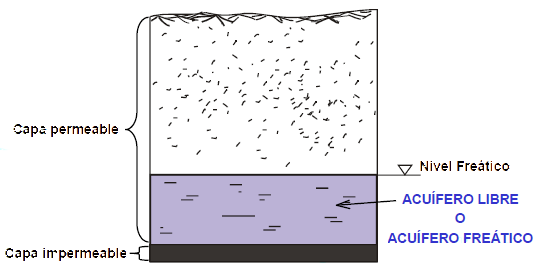
\includegraphics[width=7cm]{../img/libre}
			\end{center}
		\end{frame}
%  \begin{itemize}
%  \item<1-> Transformada de Hough
%  \item<2-> Histograma
%  \end{itemize}

\subsection{Acuífero confinado}
	\begin{frame}{Acuífero Confinado}
	\begin{itemize}
		\item El caso del problema:
		\begin{center}
			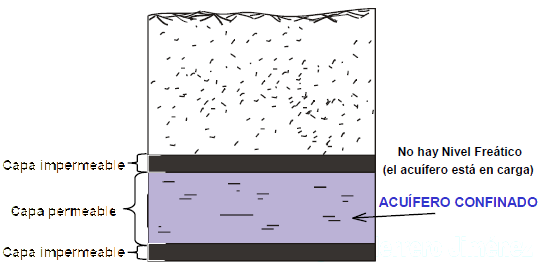
\includegraphics[width=7cm]{../img/confinado}
		\end{center}
		\item Homogéneo
		\item Isótropo
	\end{itemize}
	\end{frame}
%
%%%%%%%%%%%%%%%%%%%%%%%%%%%%%%%%%%%%%%%%%%%%%%%%%%%%%%%%%
\section{Base Teórica}
%
	\subsection{Ec. de Navier-Stokes}
		\begin{frame}{Ecuación de Navier-Stokes}
		\begin{itemize}
\item \emph{Tdyn} $\rightarrow$ basado en la solución numérica de las ecuaciones de \emph{Navier-Stokes} empleando el \emph{FEM}.		
\item \emph{Tdyn} $\rightarrow$ resuelve las ecuaciones de Navier-Stokes en tres dimensiones para un fluido incompresible o ligeramente compresible de un dominio $\Omega$ dado y un intervalo de tiempo $(0,t):$
		\end{itemize}
	\end{frame}
	\begin{frame}
\begin{eqnarray}
\label{ecns1}
\rho \left(\frac{\partial u}{\partial t}+\left( u \bullet  \nabla \right)u \right)+ \nabla p - \nabla \bullet(\mu \nabla u) &=& \rho f~ \mbox{ en  }\Omega \times (0,t)\\
\nabla \bullet u&=&0 ~ \mbox{ en  } \Omega \times (0,t)
\label{ecns2}
\end{eqnarray}
\begin{itemize}
\item $u = u(x,t):$ denota el vector velocidad,
\item $p=p(x,t)$ el campo de presiones, 
\item $\rho$ la densidad (constante), 
\item $\mu$ la viscosidad dinámica del fluido y 
\item $f$ la aceleración volumétrica.
\end{itemize}
\end{frame}
%
\begin{frame}
Las Ec. (\ref{ecns1}) y (\ref{ecns2}) necesitan ser combinadas con las siguientes condiciones de borde:
\begin{eqnarray}
u &=& u_c \mbox{ en  } \Gamma_D \times (0,t);\\
p &=& p_c \mbox{ en  } \Gamma_P \times (0,t);\\
n \cdot \sigma \cdot g_1=0 \mbox{, } n \cdot \sigma \cdot g_2=0~ \mbox{, } n \cdot u&=&u_M \mbox{ en  } \Gamma_M \times (0,t);\\
u(x,0)&=&u_0(x) \mbox{ en  } \Omega_D \times \lbrace 0 \rbrace ;\\
p(x,0)&=&p_0(x) \mbox{ en  } \Omega_D \times \lbrace 0 \rbrace ;
\end{eqnarray}
\end{frame}
%
\begin{frame}
\begin{itemize} 
\item $\Gamma = \partial \Omega$ denota la frontera del dominio $\Omega$, siendo $n$ el vector normal unitario 
\item $g_1$, $g_2$ los vectores tangentes de la frontera $\partial \Omega$,
\item $u_c$ es el campo de velocidad sobre $\Gamma_D$,
\item $p_c$ la presión sobre $\Gamma_P$,
\item $\sigma$ es el campo de tensiones,
\item $u_M$ el valor de la velocidad normal y 
\item $u_0$, $p_0$ los campos de velocidad y presión iniciales
\item {$\Gamma_D \cup \Gamma_P \cup \Gamma_M=\Gamma$.\\ 
$\Gamma_D \cap \Gamma_P \cap \Gamma_M=\bigcirc$. , ya que un punto de la frontera puede ser parte de un único tipo de superficie, a menos que forme parte del borde entre dos de ellas.}
\end{itemize}
\end{frame}
%
\subsection{Ley de Darcy}
\begin{frame}{Ley de Darcy}
Expresa que el flujo de agua en un medio poroso, homogéneo e isotrópico es proporcional 
a la conductividad del medio poroso o conductividad hidráulica $K$ y a una fuerza conductora o gradiente hidráulico $i$.
\begin{eqnarray}
Q&=&K \frac{h_3 - h_4}{L} A = K \cdot i \cdot A \label{darcy_formula}
\end{eqnarray}
donde:
\end{frame}
\begin{frame}
\begin{itemize}
	\item[$Q=$] gasto, descarga o caudal en $m^3/s$,
	\item[$L=$] longitud en metros de la muestra, %seria la longitud del dominio nuestro.
	\item[$K=$] una constante, actualmente conocida como coeficiente de permeabilidad de Darcy, variable en función del material de la muestra, en $m/s$,
	\item[$A=$] área de la sección transversal de la muestra, en $m^2$,
	\item[$h_3=$] altura, sobre el plano de referencia que alcanza el agua en un tubo colocado a la entrada de la capa filtrante,
	\item[$h_4=$] altura, sobre el plano de referencia que alcanza el agua en un tubo colocado a la salida de la capa filtrante,
	\item[$i=$] $\frac{h_3 - h_4}{L}=$ el gradiente hidráulico.
\end{itemize}
\end{frame}
\begin{frame}
%
\begin{figure}[tbhp]
\centerline{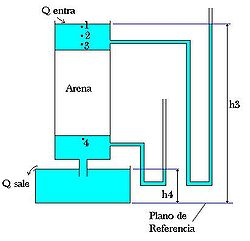
\includegraphics[scale=0.6]{../img/darcy_grafica}}
\caption{Ley de Darcy}
\label{graf_leydarcy}
\end{figure}
\end{frame}
%
\begin{frame}
\begin{itemize}
\item $K$ depende tanto del medio como del propio fluido.
\item La parte que depende del fluido, normalmente es despreciable
	\begin{itemize} 
		\item viscosidad y peso específico del \textbf{agua} varían poco con la temperatura.
	\end{itemize}
\item A efectos prácticos asumimos: \emph{conductividad hidráulica} ($K$ de Darcy) es una característica del medio poroso.
\item Cuando el valor de $K$ es muy bajo o cuando las velocidades del flujo son muy altas $\rightarrow$ la relación entre el caudal y el gradiente hidráulico no es lineal.
\item En el flujo subterráneo las velocidades son muy lentas y prácticamente siempre la relación es lineal, salvo en las proximidades de captaciones bombeando en ciertas condiciones.
\end{itemize}
\end{frame}
%%%%%%%%%%%%%%%%%%%%%%%%%%%%%%%%%%%%%%%%%%%%%%%%%%%%%%%%%
\section{Desarrollo del problema}
%
\begin{frame}
\begin{itemize}
\item 2 geometrías: \emph{G1} y \emph{G2}
\item 2 simulaciones
\end{itemize}
\end{frame}
%
\subsection{Datos del problema}
\subsubsection{Geometría G1}
\begin{frame}{Geometría G1}
\begin{itemize}
	\item Discretización del área a modelar:	
	\begin{itemize}
		\item \textbf{Dominio: $x=100 ~\left[m\right]$, $y=100 ~\left[m\right]$}
		\item Acuífero confinado, homogéneo e isótropo $(K_{xx} = K_{yy} = K_{zz})$
		\item Espesor del acuífero: $20 ~\left[m\right]$
	\end{itemize}
	%
	\item Coordenadas de ubicación de los Pozos de bombeo:
	\begin{itemize}
		\item Pozo Bombeo 1: $x=17.5~~\left[m\right]$, $y=77.5 ~~\left[m\right]$
		\item Pozo Bombeo 2: $x=65.0~~\left[m\right]$, $y=22.5 ~~\left[m\right]$
	\end{itemize}
	%
	\item Caudal de bombeo:
	\begin{itemize}
		\item Pozo Bombeo 1: $60~\left[\frac{m^3}{h}\right]$
		\item Pozo Bombeo 2: $40~\left[\frac{m^3}{h}\right]$
	\end{itemize}
	\item Diámetro del pozo 1 y 2: $0.5 [m]$
	\item Profundidad del pozo 1 y 2: $15 [m]$
%	\item Transmisividad: $600~\left[\frac{m^2}{d}\right]$ \begin{LARGE}
%	eso no se si va!!!
%	\end{LARGE}\\
	\item Resistencia de la ley de Darcy $k=0.0000017~[1/m^2]$
\end{itemize}
\end{frame}
%
\subsubsection{Geometría G2}
\begin{frame}{Geometría G2}
\begin{itemize}
	\item Discretización del área a modelar:	
	\begin{itemize}
		\item \textbf{Dominio: $x=200 ~\left[m\right]$, $y=200 ~\left[m\right]$}
		\item Acuífero confinado, homogéneo e isótropo $(K_{xx} = K_{yy} = K_{zz})$
		\item Espesor del acuífero: $20 ~\left[m\right]$
	\end{itemize}
	%
	\item Coordenadas de ubicación de los Pozos de bombeo:
	\begin{itemize}
		\item Pozo Bombeo 1: $x=30.0 ~~\left[m\right]$, $y=135.0 ~~\left[m\right]$
		\item Pozo Bombeo 2: $x=150.0~~\left[m\right]$, $y=50.0 ~~\left[m\right]$
	\end{itemize}
	%
	\item Caudal de bombeo:
	\begin{itemize}
		\item Pozo Bombeo 1: $60~\left[\frac{m^3}{h}\right]$
		\item Pozo Bombeo 2: $40~\left[\frac{m^3}{h}\right]$
	\end{itemize}
	\item Diámetro del pozo 1 y 2: $0.5 [m]$
	\item Profundidad del pozo 1 y 2: $15 [m]$
%	\item Transmisividad: $600~\left[\frac{m^2}{d}\right]$ \begin{LARGE}
%	eso no se si va!!!
%	\end{LARGE}\\
	\item Resistencia de la ley de Darcy $k=0.0000017~[1/m^2]$
\end{itemize}
\end{frame}
%
\subsection{Relación Caudal - Velocidad}
\begin{frame}{``Caudal volumétrico"}
\begin{equation}
Q=V \cdot S
\label{caudal}
\end{equation}
\begin{itemize}
\item $Q$ es el caudal,
\item $V$ es la velocidad y 
\item $S$ es la sección de la tubería
\end{itemize}
Caudal de bombeo:
	\begin{itemize}
		\item Pozo Bombeo 1: $60~\left[\frac{m^3}{h}\right] \Longrightarrow V=0.085$
		\item Pozo Bombeo 2: $40~\left[\frac{m^3}{h}\right] \Longrightarrow V=0.057$
	\end{itemize}
\end{frame}
%%%%%%%%%%%%%%%%%%%%%%%%%%%%%%%%%%%%%%%%%%%%%%%%%%%%%%%%%
\subsection{Propiedades del medio y de los Materiales}
\subsubsection{Material Suelo}
\begin{frame}
\begin{itemize}
\item Modelo de Fluido: flujo incompresible ($\rho = cte.$)
\item Densidad: $999.7~Kg/m^3$ (agua a $10$\grad$C$)
\item Viscosidad: $0.001307~Pa.s$ (agua a $10$\grad$C$)
\item Resistencia de la Ley de Darcy:
\begin{equation}
\begin{pmatrix}{}
0.0000017 & 0.0 & 0.0 \\ 
0.0 & 0.0000017 & 0.0 \\ 
0.0 & 0.0 & 0.0000017
\end{pmatrix} [1/m^2]
\label{matrizdarcys}
\end{equation}
\item acuífero isótropo (homogéneo en todo el suelo)
\end{itemize}
\end{frame}
%
\begin{frame}
\begin{center}
\begin{figure}[tbhp]
\centerline{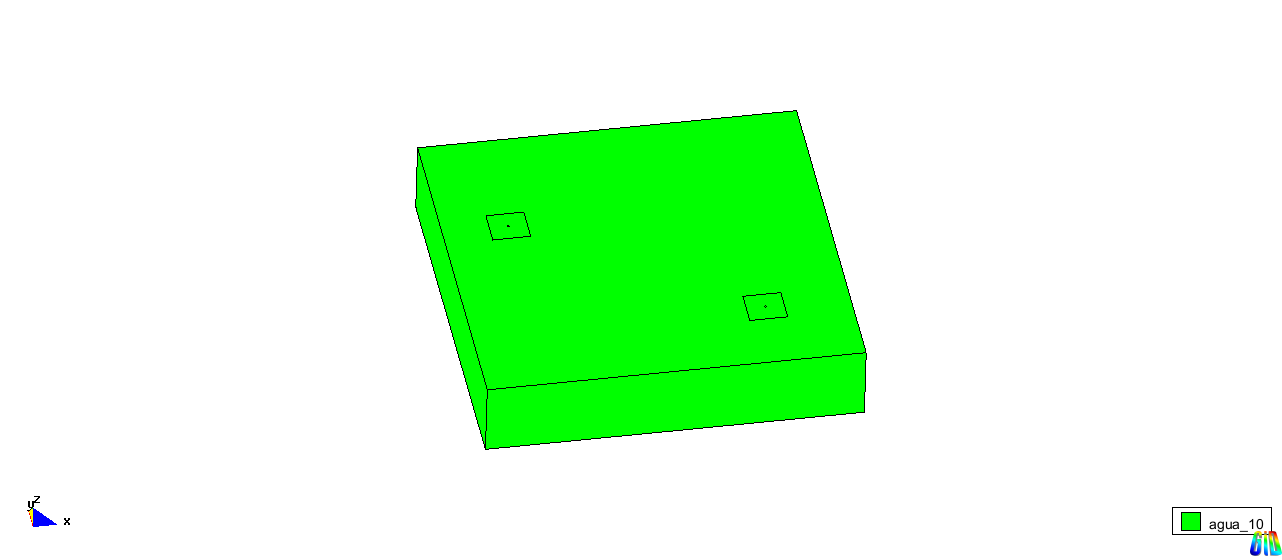
\includegraphics[scale=0.4]{../img/100m/100_perspectiva_material_agua}}
\caption{Material Suelo asignado a la geometría}
\label{100_perspectiva_material_agua}
\end{figure}
\end{center}
\end{frame}
%
\subsubsection{Material Wall o Pared}
\begin{frame}
V fixWall
\begin{center}
\begin{figure}[tbhp]
\centerline{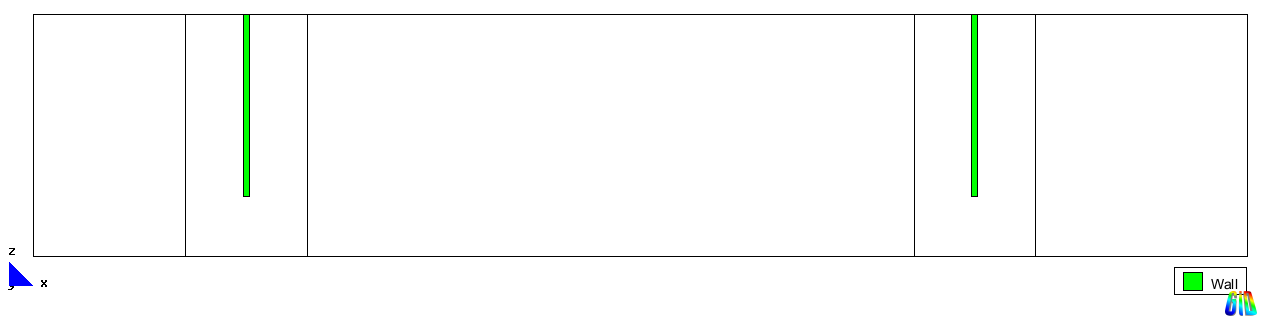
\includegraphics[scale=0.25]{../img/100m/100_condiciones_vfixwall_xz}}
\caption{Material Wall o Pared asignado a la geometría}
\label{100_condiciones_vfixwall_xz}
\end{figure}
\end{center}
\end{frame}
%%%%%%%%%%%%%%%%%%%%%%%%%%%%%%%%%%%%%%%%%%%%%%%%%%%%%%%%%
\subsection{Condiciones de Borde}
\subsubsection{Fijar Velocidad}
\begin{frame}\begin{center}
\begin{figure}[tbhp]
\centerline{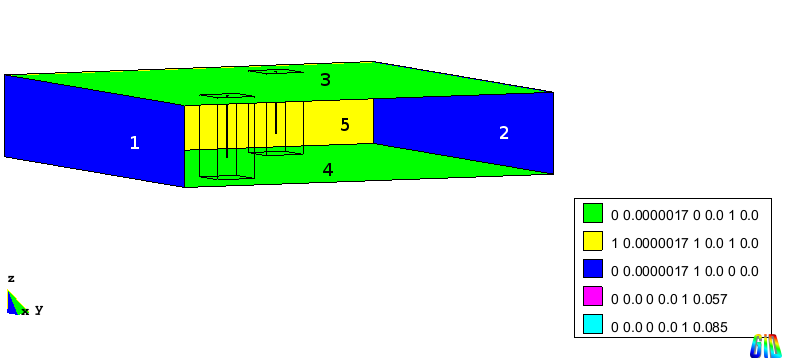
\includegraphics[scale=0.4]{../img/100m/100_condiciones_fijar_velocidad_perspectiva_interior_leyendas}}
\caption{Velocidades Fijas}
\label{100_condiciones_fijar_velocidad_perspectiva_interior_leyendas}
\end{figure}
\end{center}
\end{frame}
%
\begin{frame}\begin{center}
\begin{figure}[htbp] 
\centering 
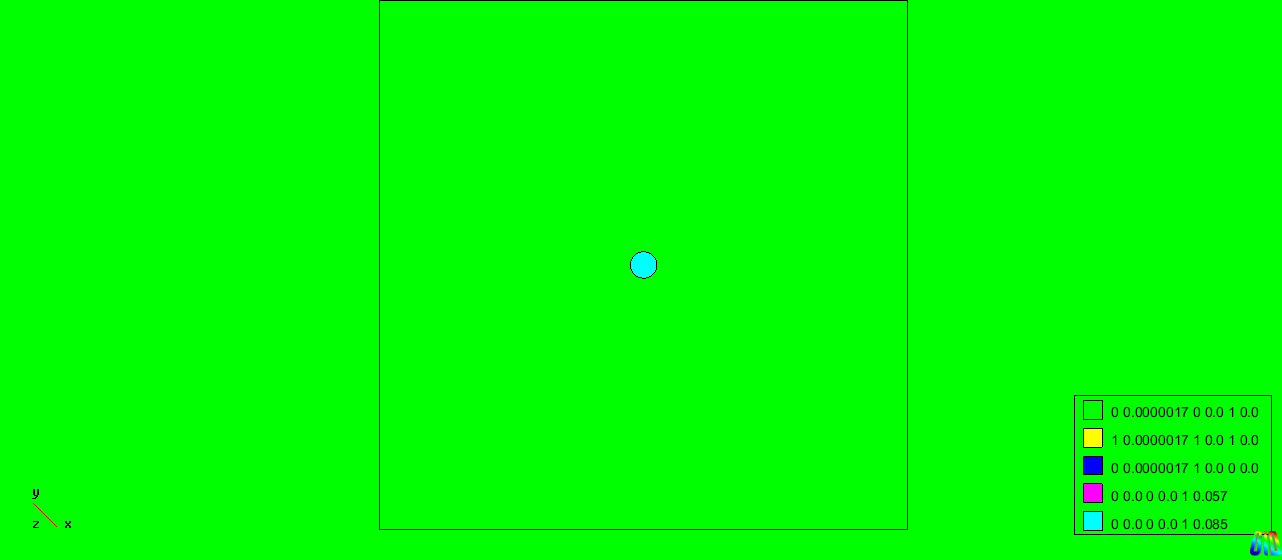
\includegraphics[scale=0.18]{../img/100m/100_condiciones_fijar_velocidad_fondo_pozos_arriba_izquierda} 
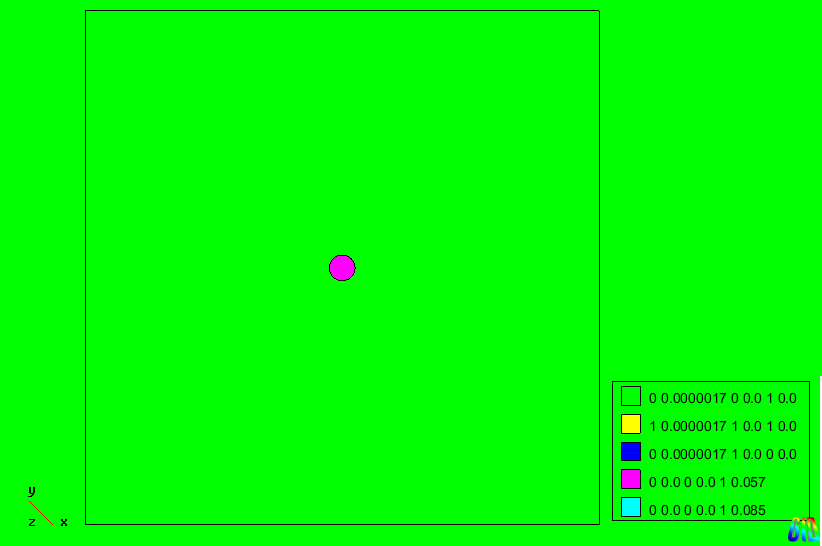
\includegraphics[scale=0.18]{../img/100m/100_condiciones_fijar_velocidad_fondo_pozos_abajo_derecha}
%\caption{Vista en detalle de la Figura (\ref{100_condiciones_fijar_velocidad_perspectiva_interior_leyendas})} 
\label{fondo_pozos_detalles} 
\end{figure} 
\end{center}
\end{frame}
\subsubsection{Fijar Presión}
\begin{frame}\begin{center}
\begin{figure}[tbhp]
\centerline{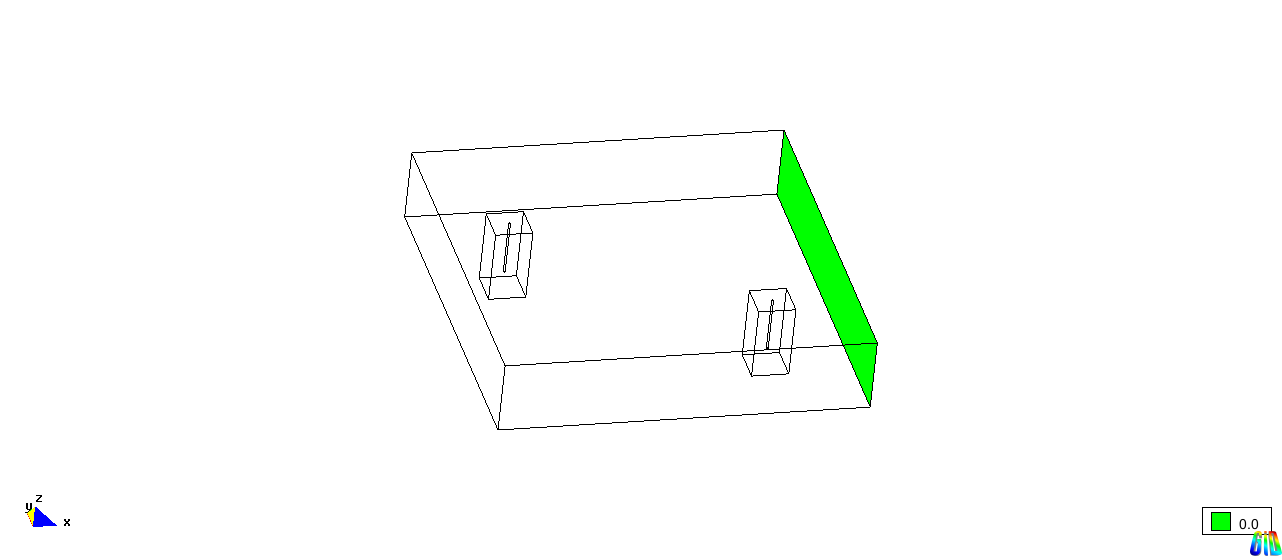
\includegraphics[scale=0.4]{../img/100m/100_condiciones_presion0}}
\caption{Condición fija de presión}
\label{100_condiciones_presion0}
\end{figure}
\end{center}
\end{frame}
%%%%%%%%%%%%%%%%%%%%%%%%%%%%%%%%%%%%%%%%%%%%%%%%%%%%%%%%%
\subsection{Mallado}
\begin{frame}{G1}\begin{center}
\begin{itemize}
\item Transición de tamaños no estructurados $=0.3$.
\end{itemize}
\begin{figure}[tbhp]
\centerline{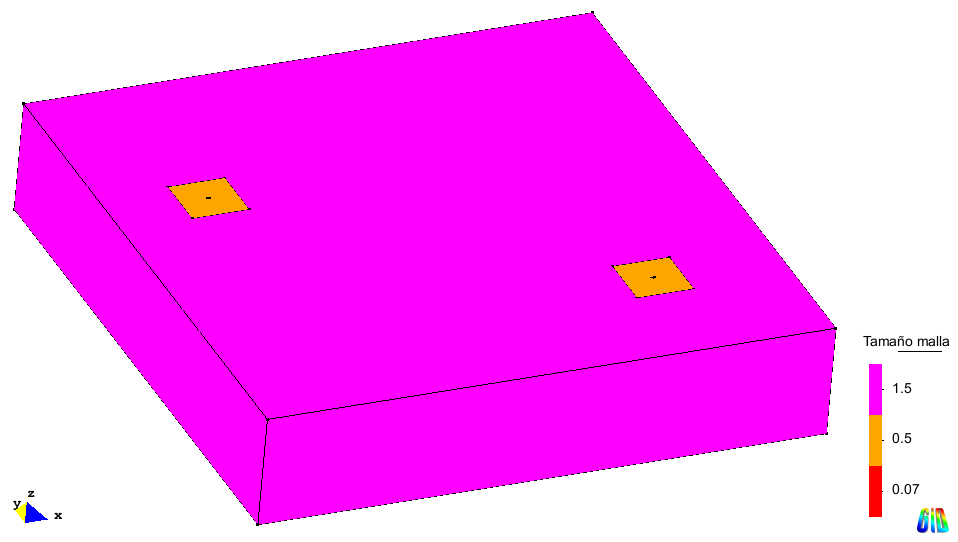
\includegraphics[scale=0.21]{../img/100m/100_perspec_tam_malla}}
\caption{Tamaños de los elementos de la malla \emph{G1}- Vista en perspectiva}
\label{100_perspec_tam_malla}
\end{figure}
\end{center}\end{frame}
%
\begin{frame}{G1}\begin{center}
\begin{figure}[tbhp]
\centerline{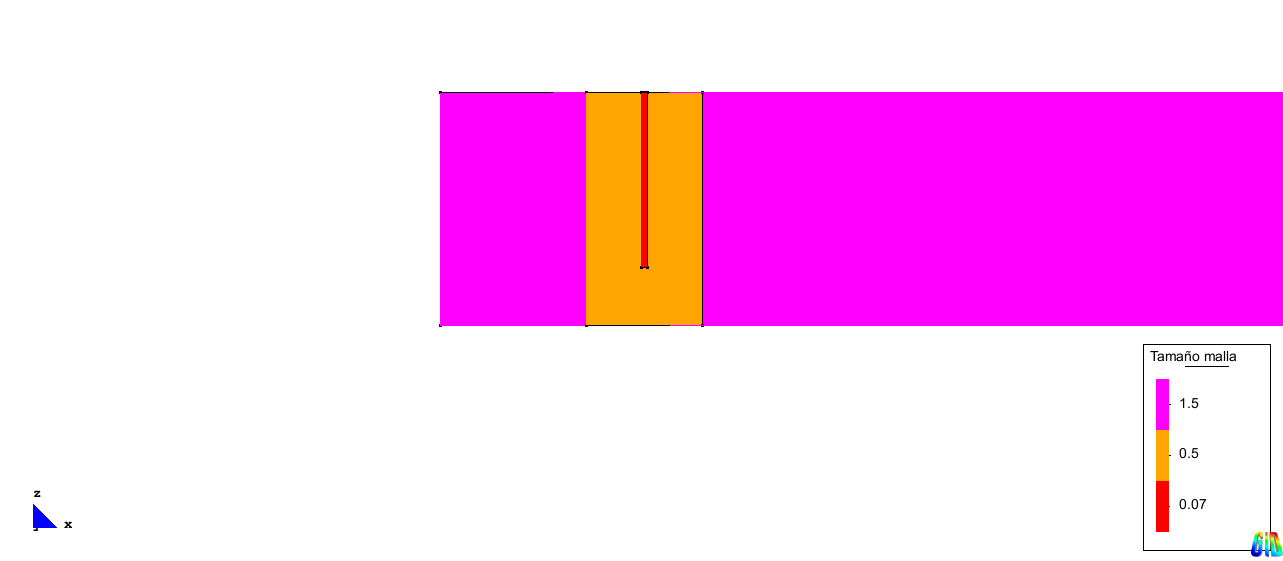
\includegraphics[scale=0.23]{../img/100m/100_xz_tam_malla}}
\caption{Tamaños de los elementos de la malla \emph{G1}- Vista plano XZ}
\label{100_xz_tam_malla}
\end{figure}
\end{center}\end{frame}
%%%%%%%
\begin{frame}{G2}\begin{center}
\begin{itemize}
\item Transición de tamaños no estructurados $=0.3$.
\end{itemize}
\begin{figure}[tbhp]
\centerline{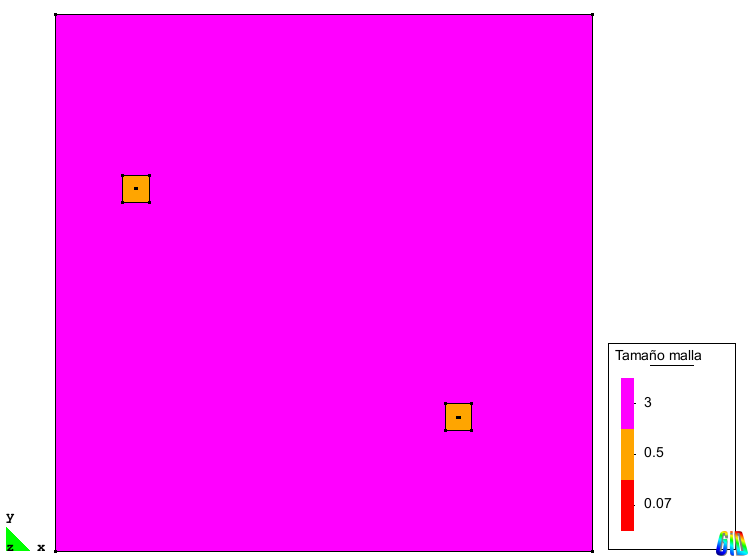
\includegraphics[scale=0.21]{../img/200m/200_xy_tam_malla}}
\caption{Tamaños de los elementos de la malla para \emph{G2}- Vista plano XY}
\label{200_xy_tam_malla}
\end{figure}
\end{center}\end{frame}
%
\begin{frame}{G2}\begin{center}
\begin{figure}[tbhp]
\centerline{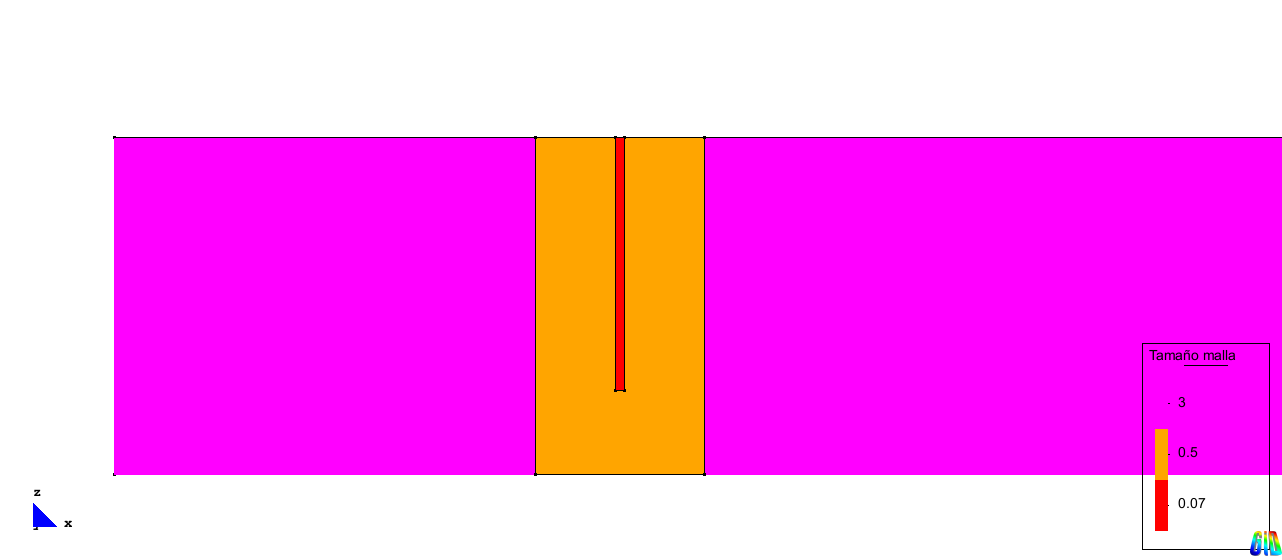
\includegraphics[scale=0.22]{../img/200m/200_xz_tam_malla}}
\caption{Tamaños de los elementos de la malla \emph{G2}- Vista plano XZ}
\label{200_xz_tam_malla}
\end{figure}
\end{center}\end{frame}
\begin{frame}
\begin{table}[tbhp]
\begin{center}\begin{tabular}{ccc}
\hline \textbf{Tipo/Geometría} & \textbf{G1} & \textbf{G2} \\ 
\hline Número de nodos: & 122586 & 157619 \\ 
\hline Número de tetraedros: & 659027 & 851671\\ 
\hline Número de triángulos: & 60952  & 70582 \\ 
\hline Número de elementos totales: & 719979 & 922253 \\ 
\hline 
\end{tabular}\end{center}
\caption{Cantidad de nodos, tetraedros, triángulos y elementos totales para \emph{G1} y \emph{G2}}
\label{tabla_lista_elementos}
\end{table}
\end{frame}
%
\begin{frame}{Malla para G1}\begin{center}
\begin{figure}[tbhp]
\centerline{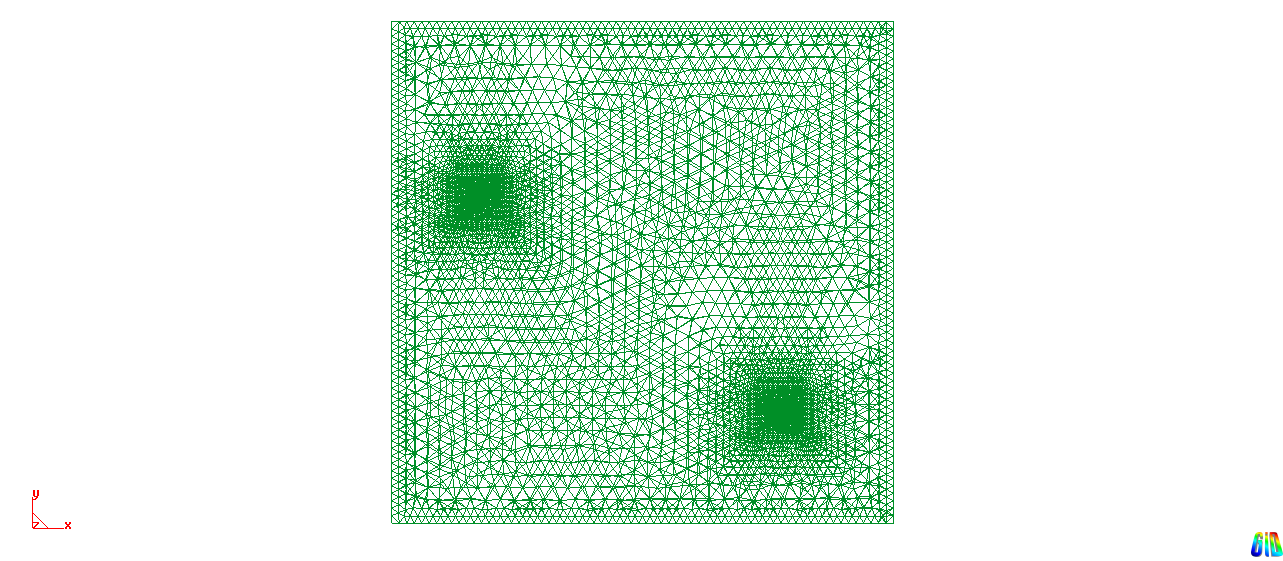
\includegraphics[scale=0.25]{../img/100m/100_xy_contorno_malla}}
\caption{Mallado generada para \emph{G1}- Vista plano XY}
\label{100_xy_contorno_malla}
\end{figure}
\end{center}\end{frame}
%
\begin{frame}{Malla para G2}\begin{center}
\begin{figure}[tbhp]
\centerline{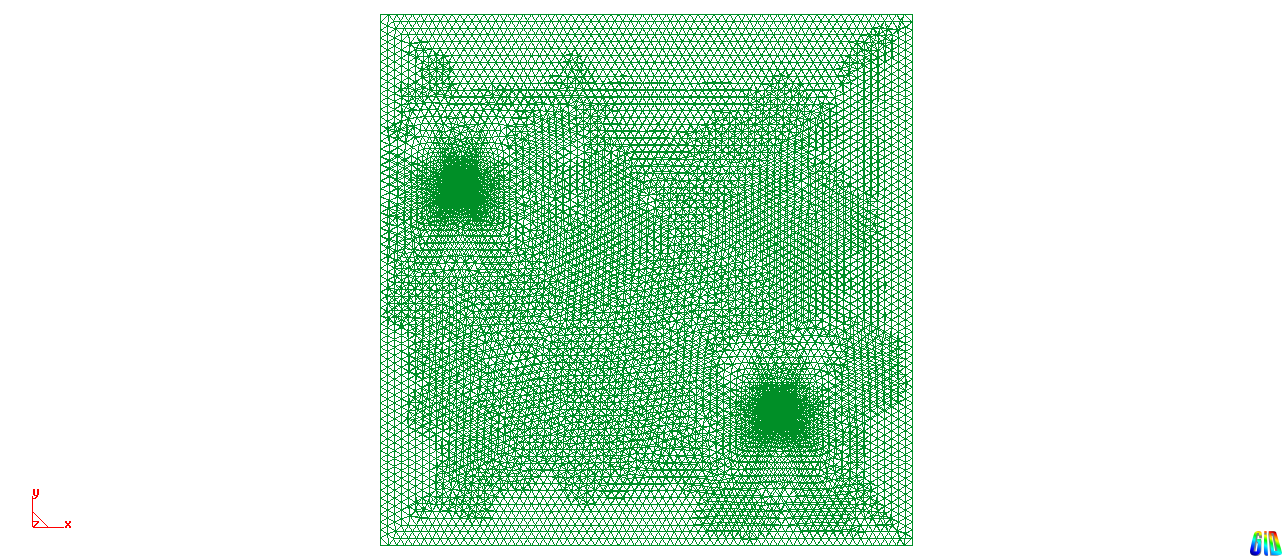
\includegraphics[scale=0.25]{../img/200m/200_xy_contorno_malla}}
\caption{Mallado generada para \emph{G2}- Vista plano XY}
\label{200_xy_contorno_malla}
\end{figure}
\end{center}\end{frame}
%%%%%%%%%%%%%%%%%%%%%%%%%%%%%%%%%%%%%%%%%%%%%%%%%%%%%%%%%
\subsection{Ejecución}
\begin{frame}
\begin{itemize}
\item 1000 pasos
\item $\Delta t=10~[s]$
\item 2 h., 46 m., 40 seg.
\end{itemize}
\end{frame}
%%%%%%%%%%%%%%%%%%%%%%%%%%%%%%%%%%%%%%%%%%%%%%%%%%%%%%%%%
\section{Resultados}
%
\subsection{Resultados para G1}
\begin{frame}{Vectores de velocidad}
\begin{center}
\begin{figure}[htbp]
\centerline{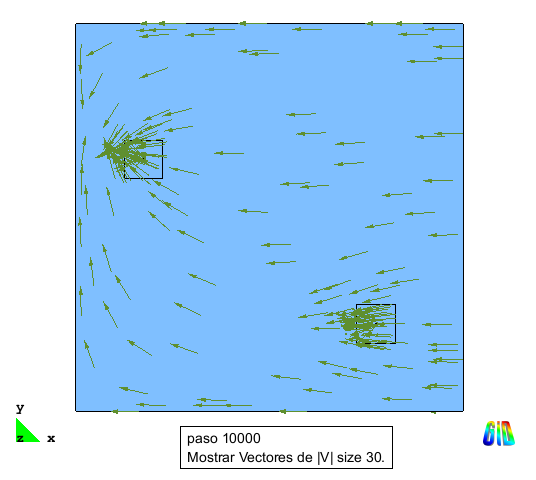
\includegraphics[scale=0.4]{../img/100m/resul/100_xy_vectores}}
\caption{Vectores para \emph{G1}- Vista plano XY}
\end{figure}
\end{center}
\end{frame}
%
\begin{frame}{Corte por el centro de los pozos}
\begin{center}
\begin{figure}[htbp]
\centerline{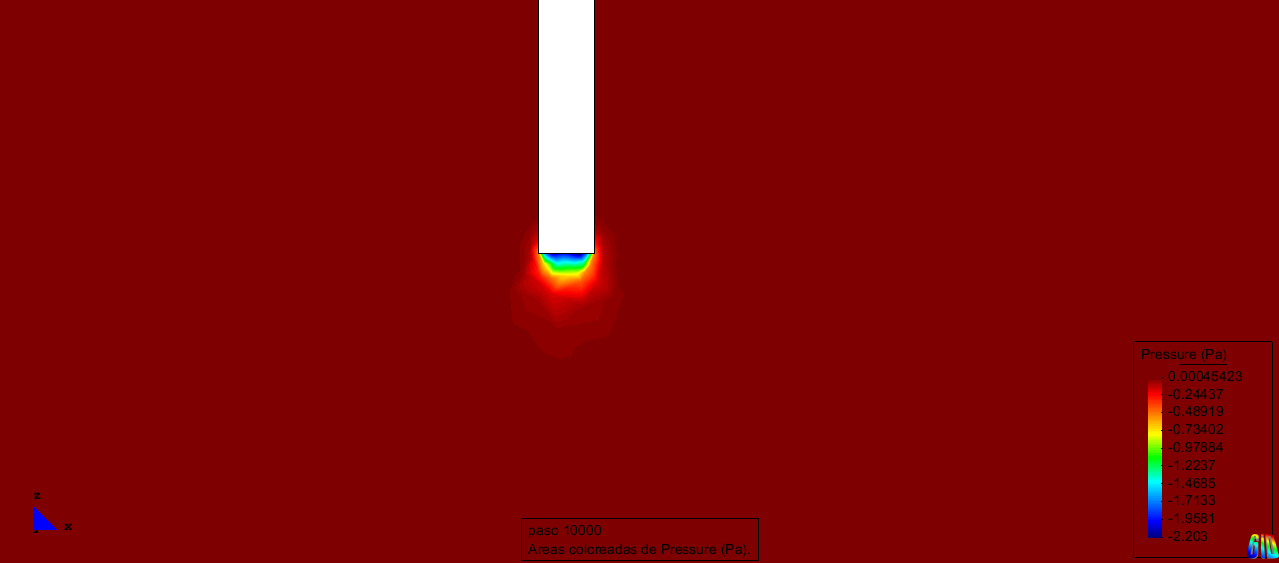
\includegraphics[scale=0.3]{../img/100m/resul/100_XZ_presion_corte_centro_pozo1}}
\caption{Presión pozo 1}
\end{figure}
\end{center}
\end{frame}
%
\begin{frame}{Corte por el centro de los pozos}
\begin{center}
\begin{figure}[htbp]
\centerline{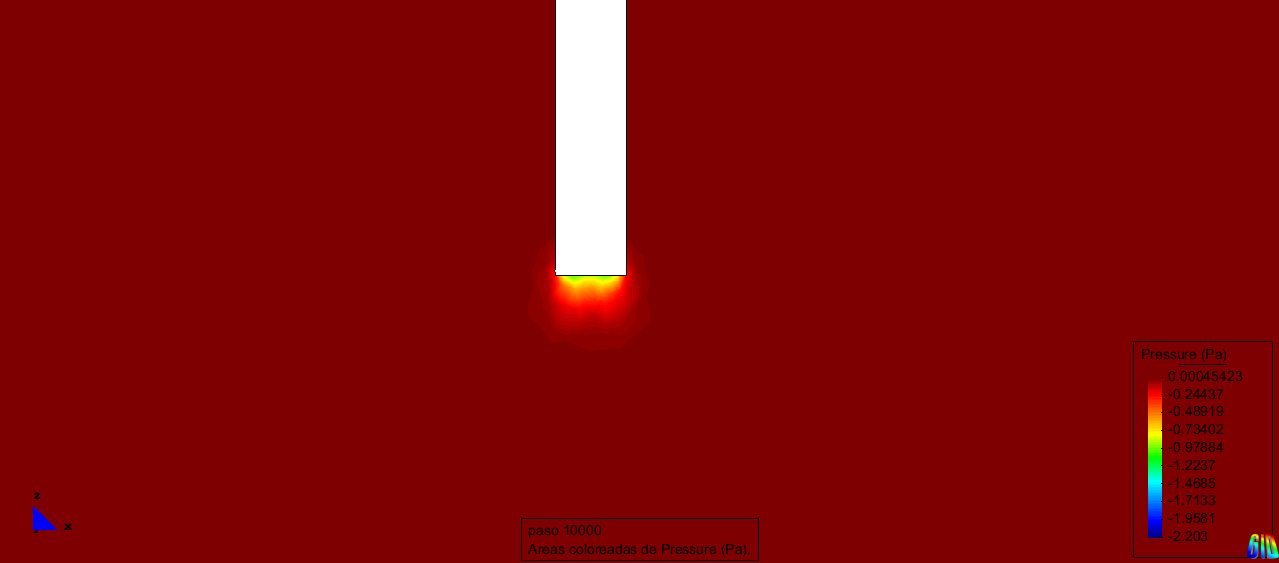
\includegraphics[scale=0.3]{../img/100m/resul/100_XZ_presion_corte_centro_pozo2}}
\caption{Presión pozo 2}
\end{figure}
\end{center}
\end{frame}
%
\begin{frame}{Corte por el centro de los pozos}
\begin{center}
\begin{figure}[htbp]
\centerline{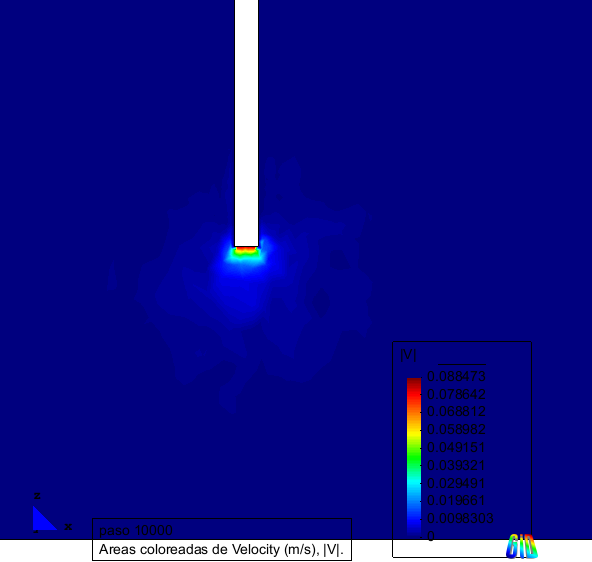
\includegraphics[scale=0.25]{../img/100m/resul/100_XZ_velocidad_corte_centro_pozo1}}
\caption{Módulo de velocidad pozo 1}
\end{figure}
\end{center}
\end{frame}
%
\begin{frame}{Corte por el centro de los pozos}
\begin{center}
\begin{figure}[htbp]
\centerline{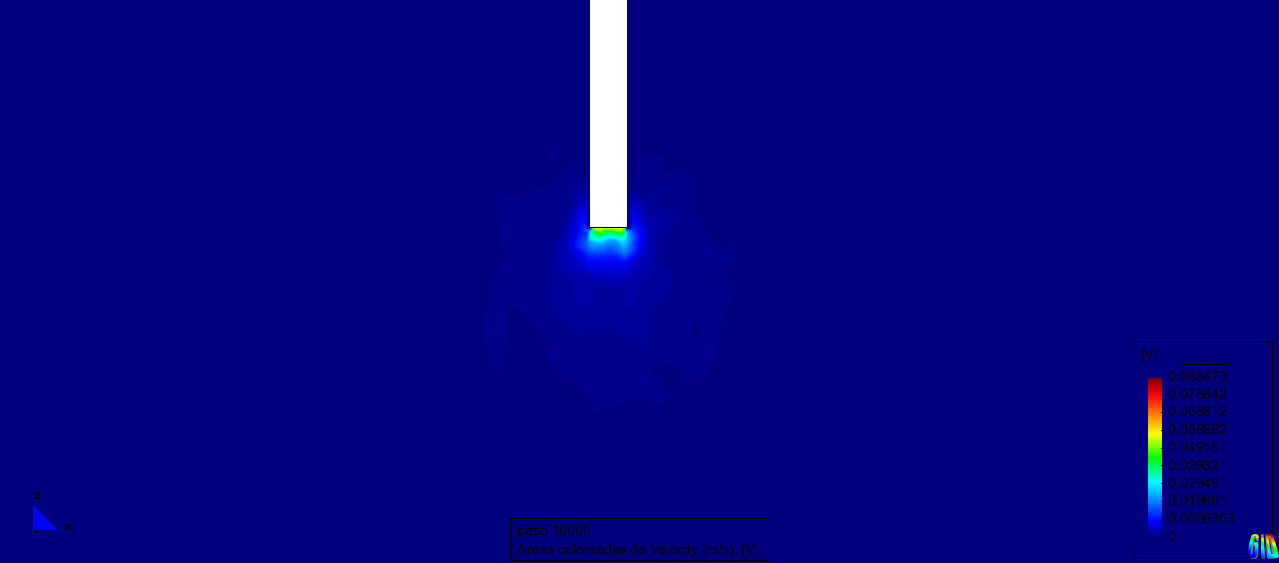
\includegraphics[scale=0.25]{../img/100m/resul/100_XZ_velocidad_corte_centro_pozo2}}
\caption{Módulo de velocidad pozo 2}
\end{figure}
\end{center}
\end{frame}
%
\begin{frame}{Corte transversal - H}
\begin{center}
\begin{figure}[htbp]
\centerline{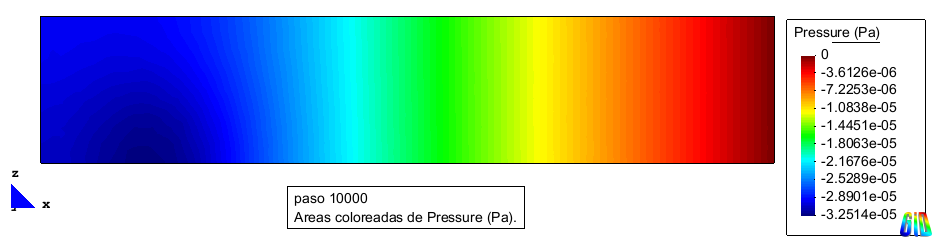
\includegraphics[scale=0.3]{../img/100m/resul/100_XZ_presion_corte_horizontal}}
\caption{Corte en $(x_1,y_1,z_1)=(0,50,0)$ hasta $(x_2,y_2,z_2)=(100,50,0)$ - Vista en el plano XZ - Presión}
\end{figure}
\end{center}
\end{frame}
%
\begin{frame}{Corte transversal - H}
\begin{center}
\begin{figure}[htbp]
\centerline{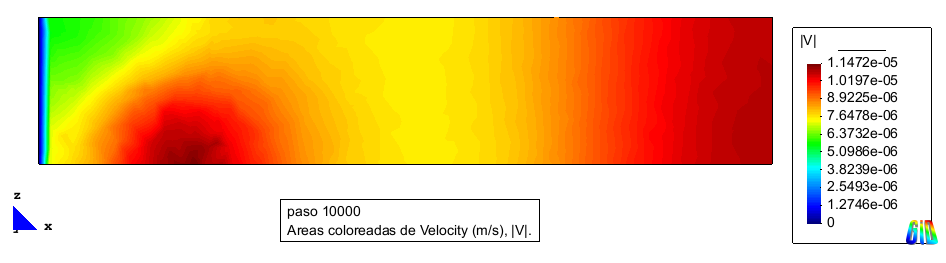
\includegraphics[scale=0.3]{../img/100m/resul/100_XZ_velocidad_corte_horizontal}}
\caption{Corte en $(x_1,y_1,z_1)=(0,50,0)$ hasta $(x_2,y_2,z_2)=(100,50,0)$ - Vista en el plano XZ - Módulo de Velocidad}
\end{figure}
\end{center}
\end{frame}
%
\begin{frame}{Corte transversal - V}
\begin{center}
\begin{figure}[htbp]
\centerline{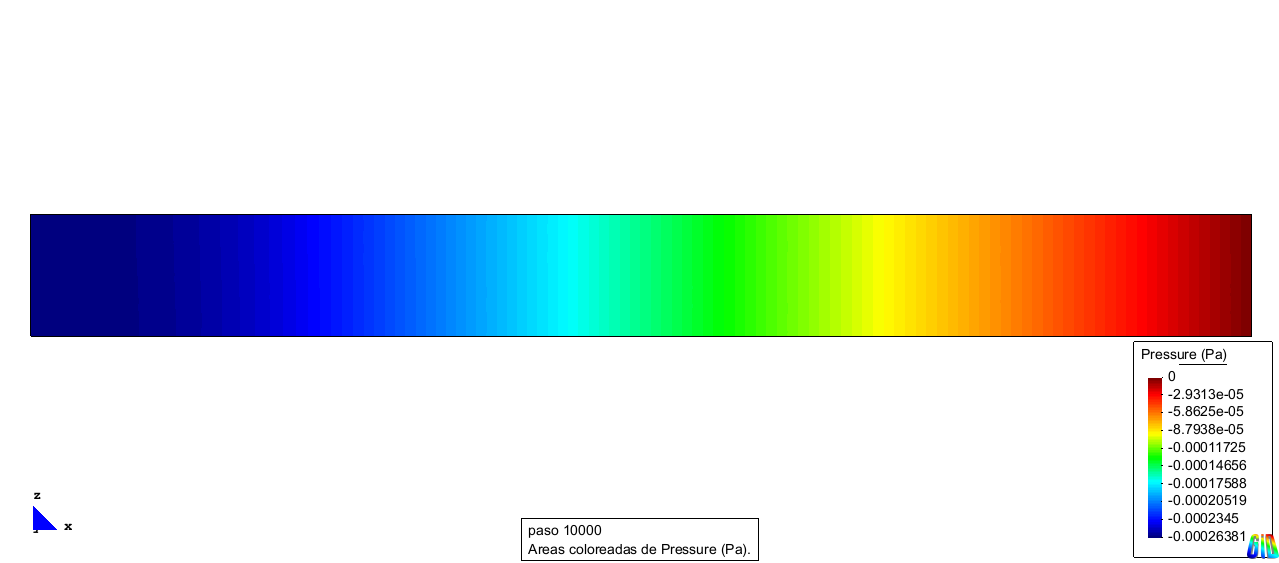
\includegraphics[scale=0.3]{../img/200m/resul/200_XZ_presion_corte_horizontal}}
\caption{Corte en $(x_1,y_1,z_1)=(50,0,0)$ hasta $(x_2,y_2,z_2)=(50,100,0)$ - Vista en el plano XZ - Presión}
\end{figure}
\end{center}
\end{frame}
%
\begin{frame}{Corte transversal - V}
\begin{center}
\begin{figure}[htbp]
\centerline{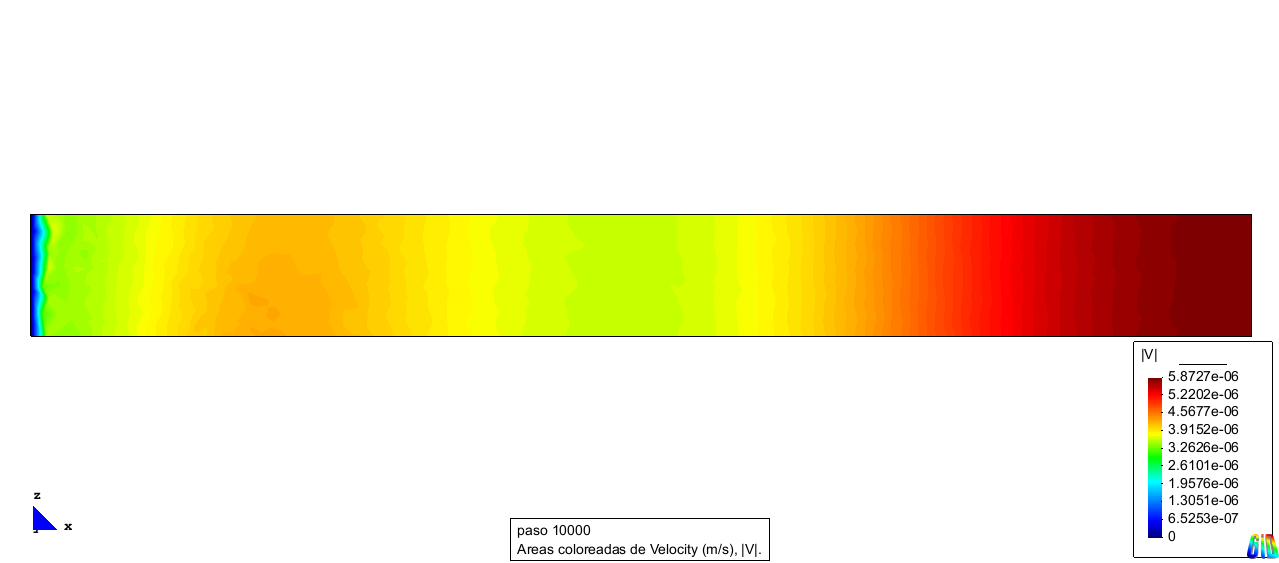
\includegraphics[scale=0.3]{../img/200m/resul/200_XZ_velocidad_corte_horizontal}}
\caption{Corte en $(x_1,y_1,z_1)=(50,0,0)$ hasta $(x_2,y_2,z_2)=(50,100,0)$ - Vista en el plano XZ - Módulo de velocidad}
\end{figure}
\end{center}
\end{frame}
%
\begin{frame}{Gráficas de borde}
\begin{center}
\begin{figure}[htbp]
\centerline{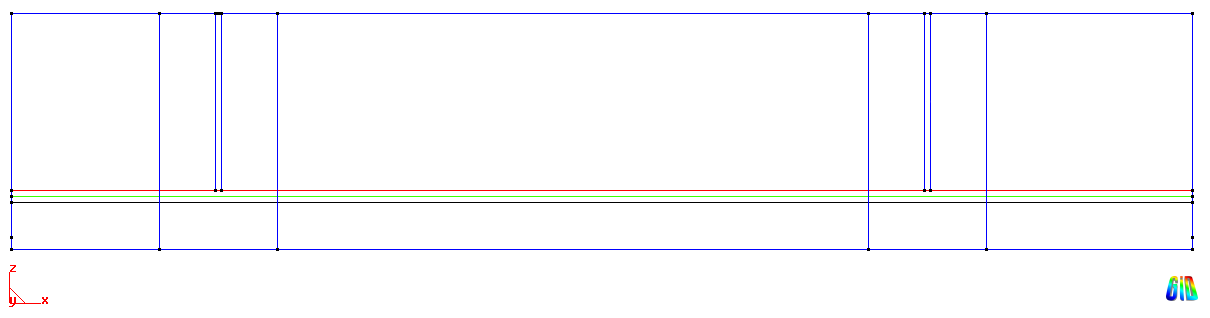
\includegraphics[scale=0.3]{../img/200m/perfiles}}
\end{figure}
\end{center}
\begin{itemize}
\item \color{red} Linea roja: situada sobre la base de los pozos
\item \color{green} Linea verde: situada a $0.5~[m]$ de la base de los pozos
\item \color{black} Linea negra: situada a $1.0~[m]$ de la base de los pozos
\end{itemize}
\end{frame}
%
\begin{frame}{Gráficas de borde situada sobre la base de los pozos}
\begin{center}
\begin{figure}[htbp]
\centerline{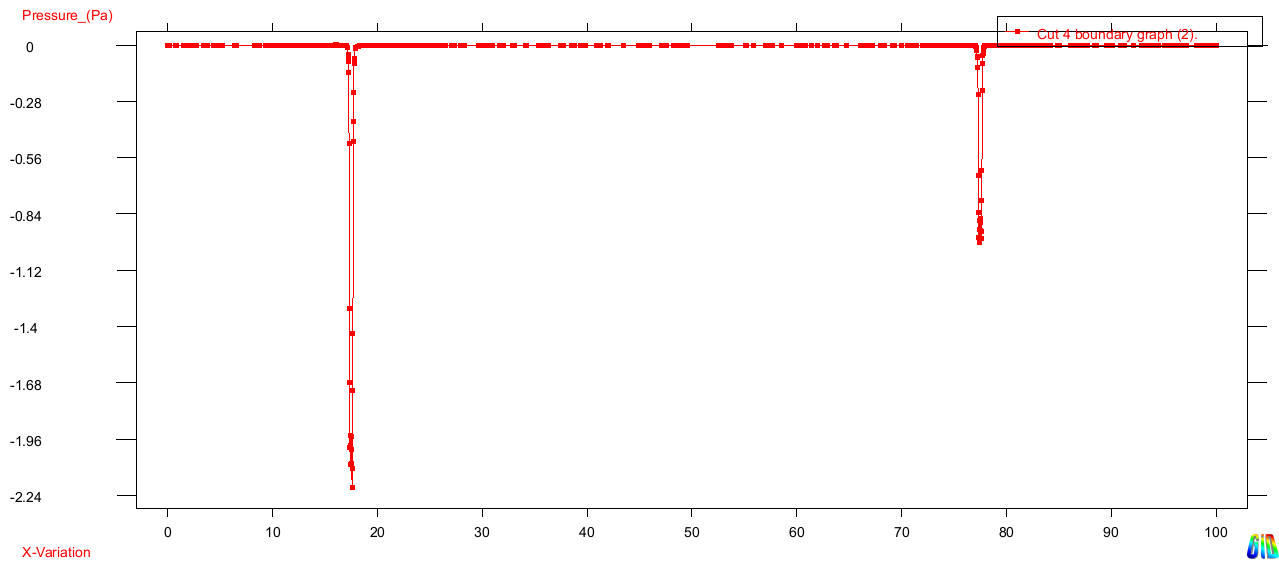
\includegraphics[scale=0.25]{../img/100m/grf/100_grafico_presion_x_centro_pozos_distancia0}}
\caption{Presión}
\end{figure}
\end{center}
\end{frame}
%
%
\begin{frame}{Gráficas de borde situada sobre la base de los pozos}
\begin{center}
\begin{figure}[htbp]
\centerline{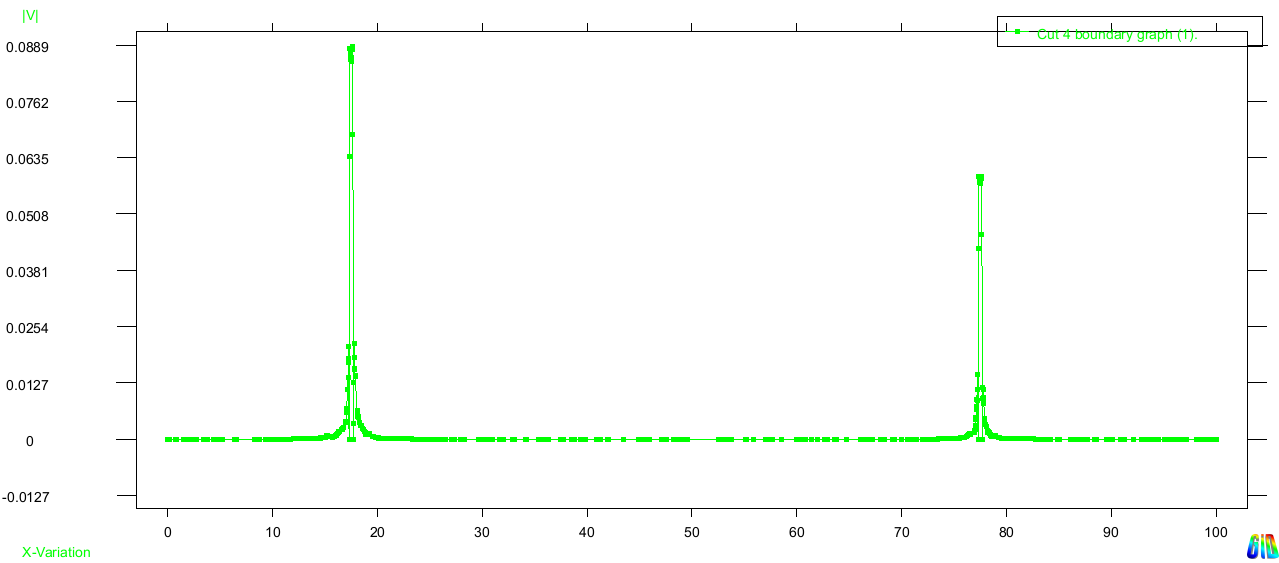
\includegraphics[scale=0.25]{../img/100m/grf/100_grafico_velocidad_x_centro_pozos_distancia0}}
\caption{Velocidad}
\end{figure}
\end{center}
\end{frame}
%
%
\begin{frame}{Gráficas de borde situada a $0.5[m]$ de la base de los pozos}
\begin{center}
\begin{figure}[htbp]
\centerline{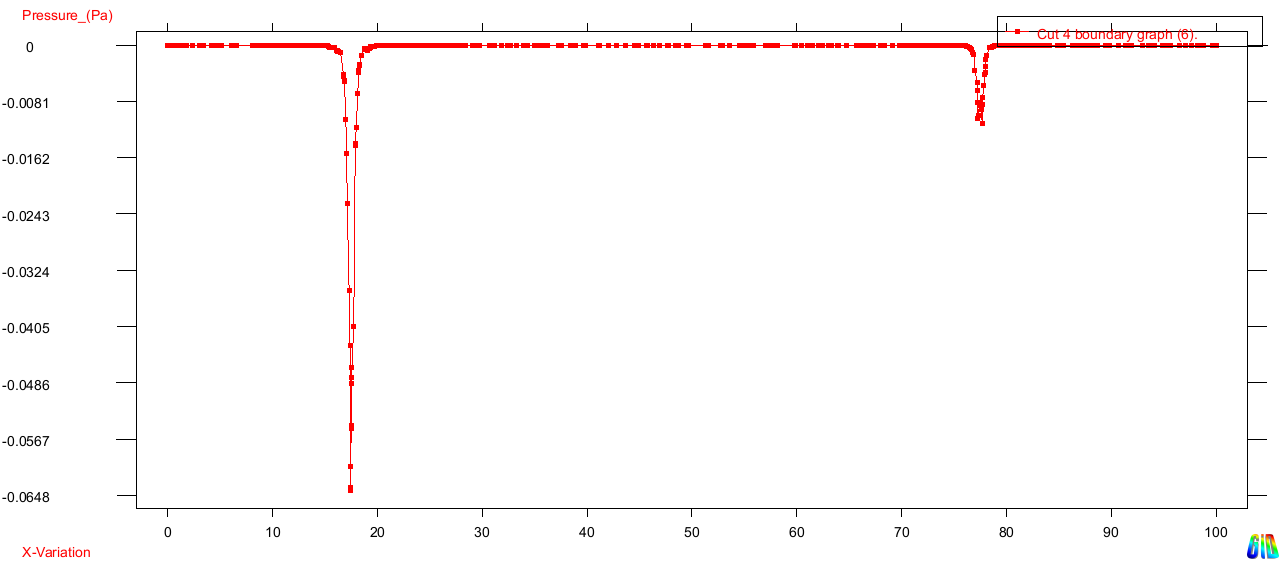
\includegraphics[scale=0.25]{../img/100m/grf/100_grafico_presion_x_centro_pozos_distancia05}}
\caption{Presión}
\end{figure}
\end{center}
\end{frame}
%
%
\begin{frame}{Gráficas de borde situada a $0.5[m]$ de la base de los pozos}
\begin{center}
\begin{figure}[htbp]
\centerline{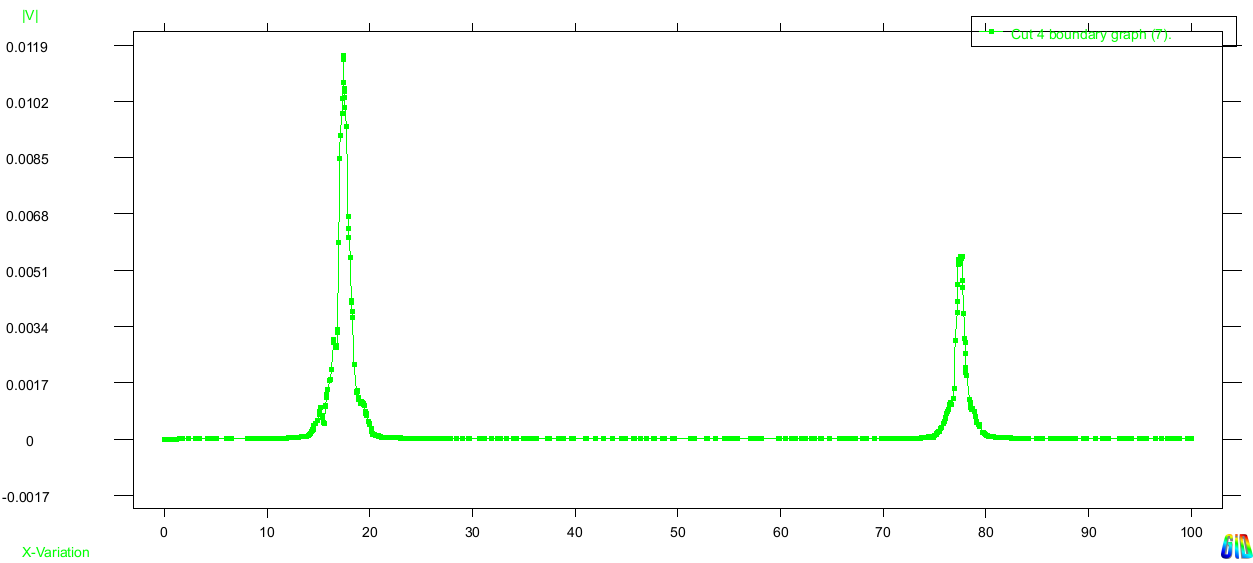
\includegraphics[scale=0.25]{../img/100m/grf/100_grafico_velocidad_x_centro_pozos_distancia05}}
\caption{Velocidad}
\end{figure}
\end{center}
\end{frame}
%
%
\begin{frame}{Gráficas de borde situada a $1.0[m]$ de la base de los pozos}
\begin{center}
\begin{figure}[htbp]
\centerline{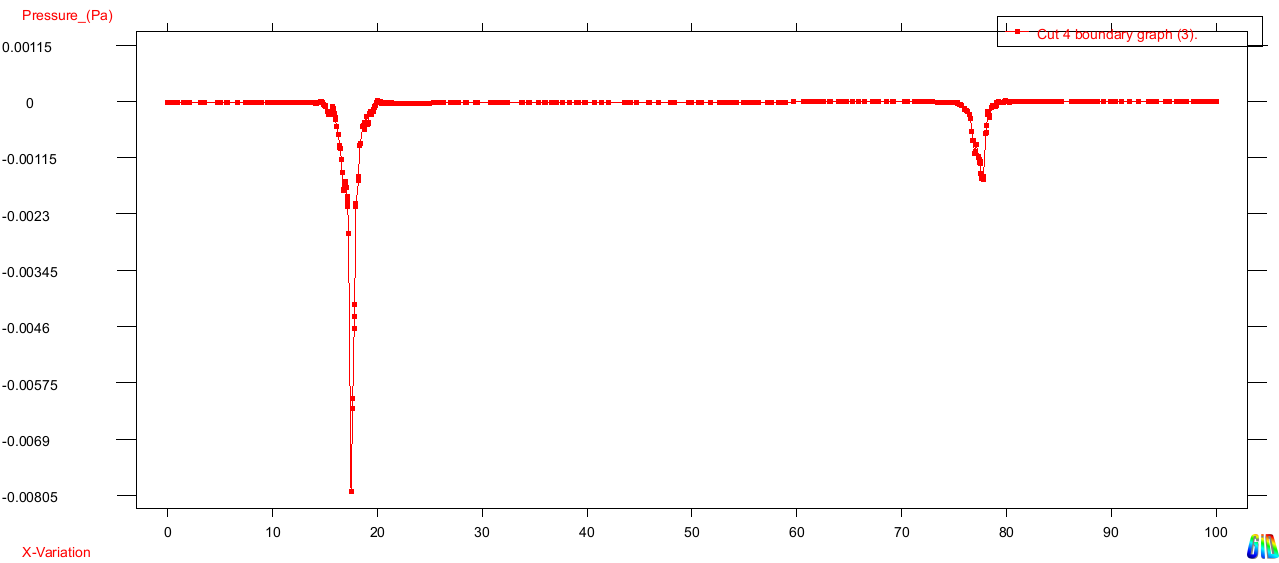
\includegraphics[scale=0.25]{../img/100m/grf/100_grafico_presion_x_centro_pozos_distancia1}}
\caption{Presión}
\end{figure}
\end{center}
\end{frame}
%
%
\begin{frame}{Gráficas de borde situada a $1.0[m]$ de la base de los pozos}
\begin{center}
\begin{figure}[htbp]
\centerline{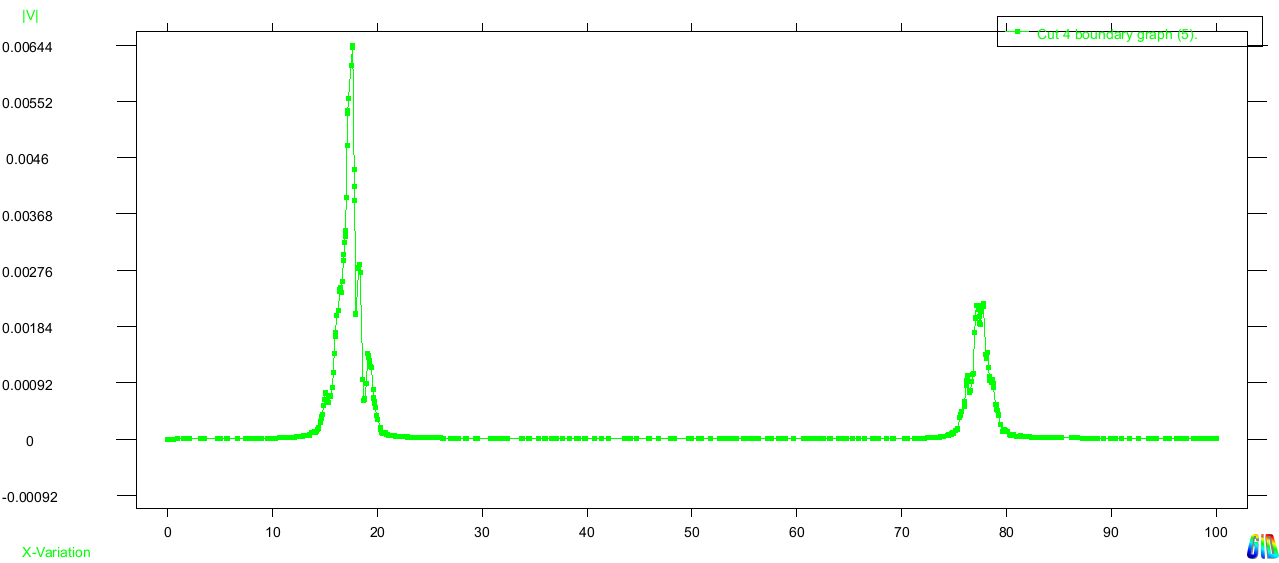
\includegraphics[scale=0.25]{../img/100m/grf/100_grafico_velocidad_x_centro_pozos_distancia1}}
\caption{Velocidad}
\end{figure}
\end{center}
\end{frame}
%
\begin{frame}
\begin{itemize}
\item a medida que se aleja de las bases de los pozos, módulo de velocidad disminuye y  la presión aumenta.
\item depresión mayor en el pozo 1 que en la base del pozo 2 $\rightarrow$ velocidades de los pozos.
\item no hay interacción notable entre los pozos $\rightarrow$ Flujo laminar y tipo de medio poroso.
\end{itemize}
\end{frame}
%%%%%%%%%%%%%%%%%%%%%%%%%%%%%%%%%%%%%%%%%%%%%
%%%%%%%%%%%%%%%%%%%%%%%%%%%%%%%%%%%%%%%%%%%%%
%
\subsection{Resultados para G2}
\begin{frame}{Vectores de velocidad}
\begin{center}
\begin{figure}[htbp]
\centerline{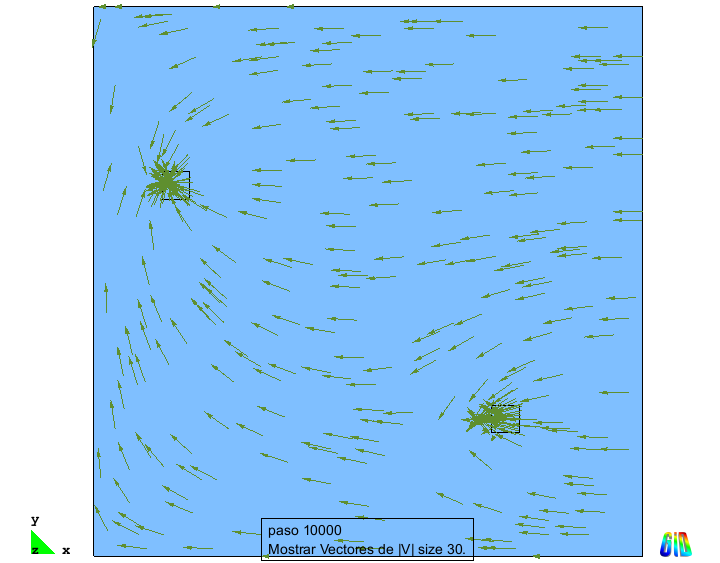
\includegraphics[scale=0.3]{../img/200m/resul/200_xy_vectores}}
\caption{Vectores para \emph{G2}- Vista plano XY}
\end{figure}
\end{center}
\end{frame}
%
\begin{frame}{Corte por el centro de los pozos}
\begin{center}
\begin{figure}[htbp]
\centerline{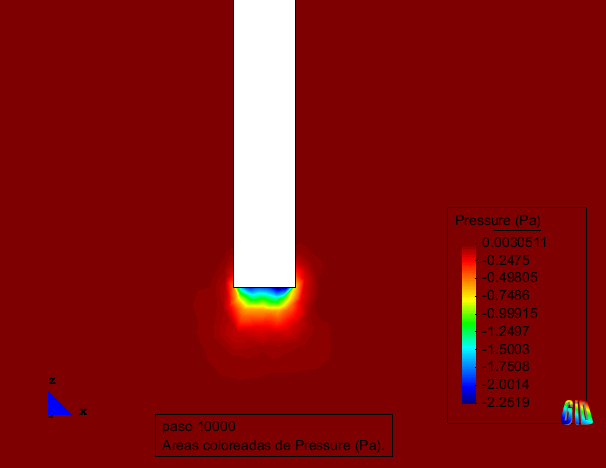
\includegraphics[scale=0.3]{../img/200m/resul/200_XZ_presion_corte_centro_pozo1}}
\caption{Presión pozo 1}
\end{figure}
\end{center}
\end{frame}
%
\begin{frame}{Corte por el centro de los pozos}
\begin{center}
\begin{figure}[htbp]
\centerline{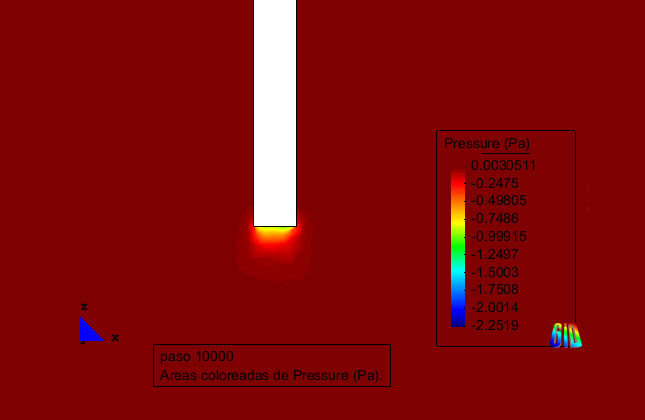
\includegraphics[scale=0.3]{../img/200m/resul/200_XZ_presion_corte_centro_pozo2}}
\caption{Presión pozo 2}
\end{figure}
\end{center}
\end{frame}
%
\begin{frame}{Corte por el centro de los pozos}
\begin{center}
\begin{figure}[htbp]
\centerline{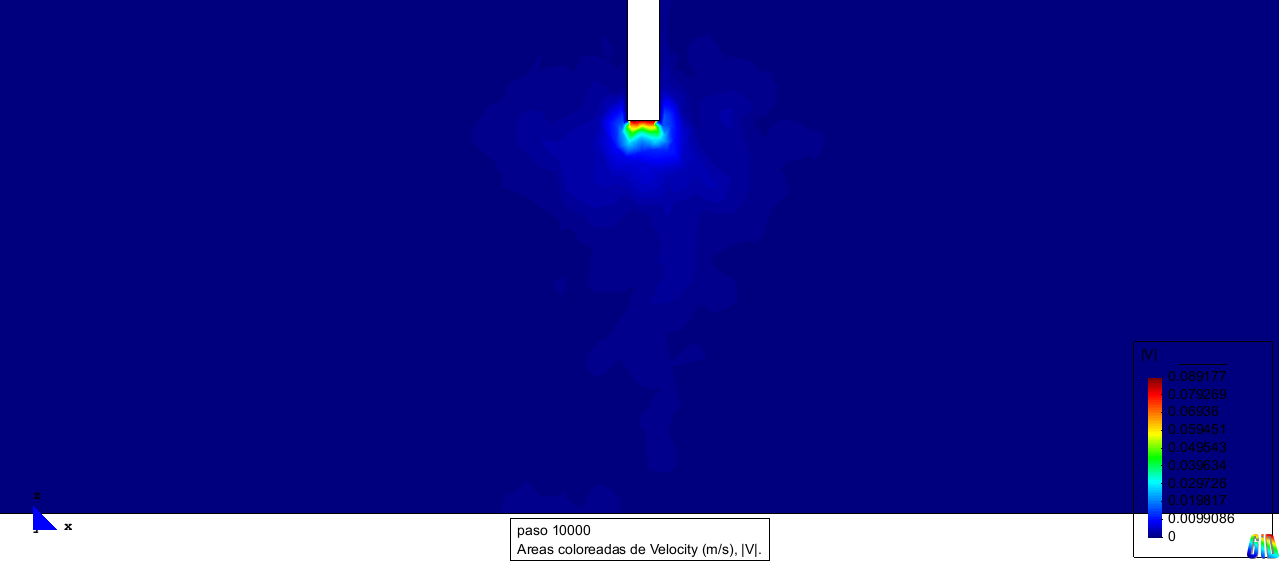
\includegraphics[scale=0.25]{../img/200m/resul/200_XZ_velocidad_corte_centro_pozo1}}
\caption{Módulo de velocidad pozo 1}
\end{figure}
\end{center}
\end{frame}
%
\begin{frame}{Corte por el centro de los pozos}
\begin{center}
\begin{figure}[htbp]
\centerline{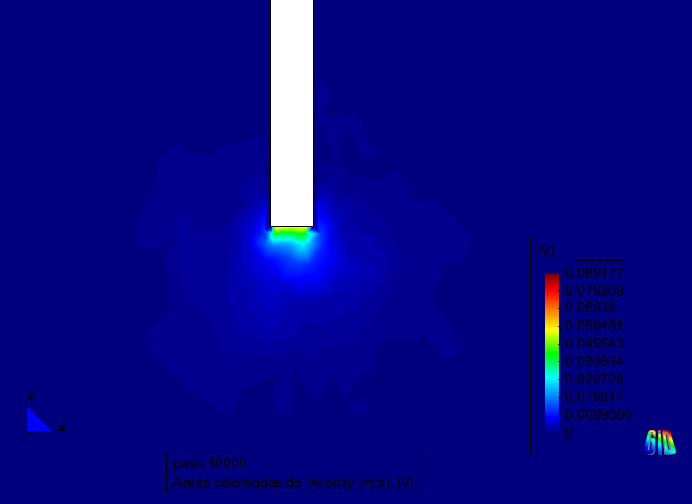
\includegraphics[scale=0.25]{../img/200m/resul/200_XZ_velocidad_corte_centro_pozo2}}
\caption{Módulo de velocidad pozo 2}
\end{figure}
\end{center}
\end{frame}
%
\begin{frame}{Corte transversal - H}
\begin{center}
\begin{figure}[htbp]
\centerline{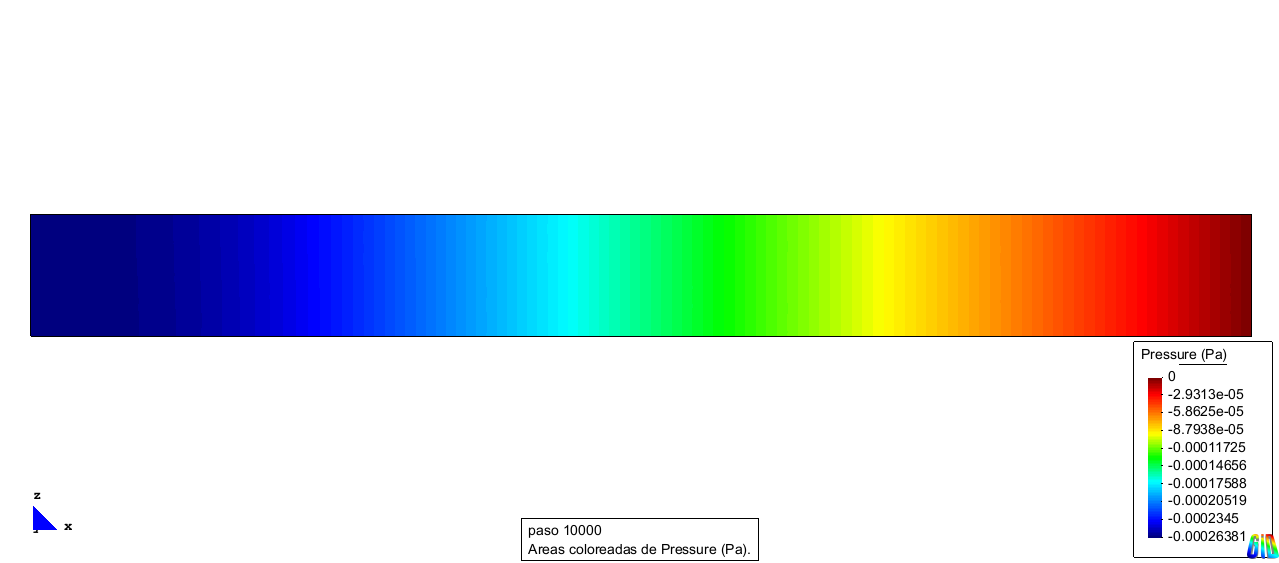
\includegraphics[scale=0.25]{../img/200m/resul/200_XZ_presion_corte_horizontal}}
\caption{Corte en $(x_1,y_1,z_1)=(0,50,0)$ hasta $(x_2,y_2,z_2)=(100,50,0)$ - Vista en el plano XZ - Presión}
\end{figure}
\end{center}
\end{frame}
%
\begin{frame}{Corte transversal - H}
\begin{center}
\begin{figure}[htbp]
\centerline{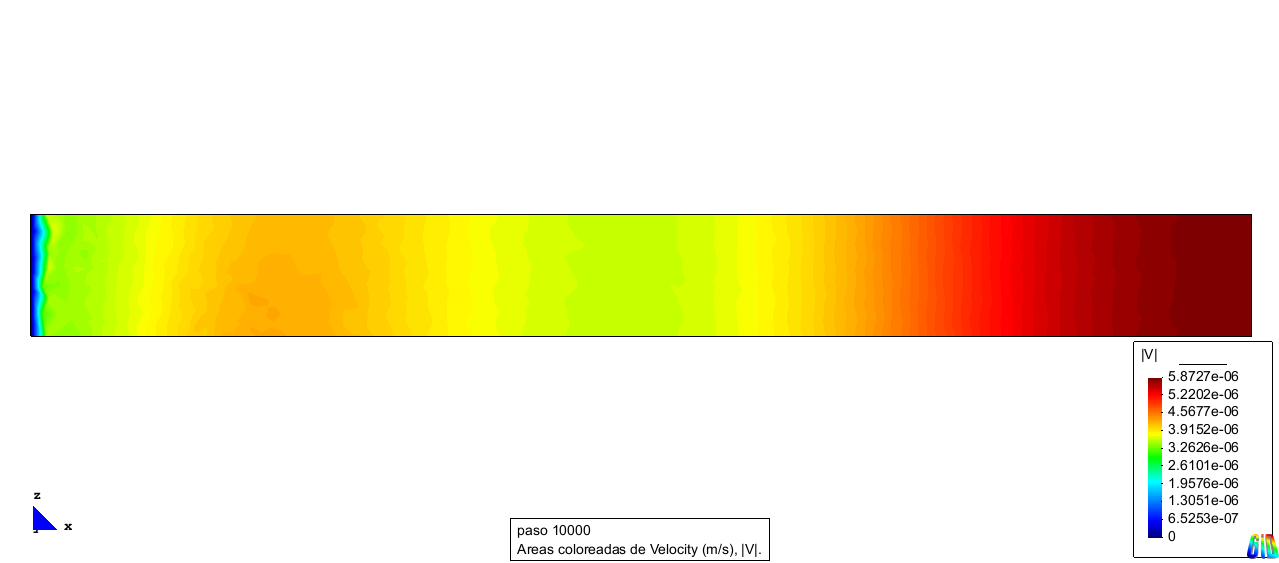
\includegraphics[scale=0.25]{../img/200m/resul/200_XZ_velocidad_corte_horizontal}}
\caption{Corte en $(x_1,y_1,z_1)=(0,50,0)$ hasta $(x_2,y_2,z_2)=(100,50,0)$ - Vista en el plano XZ - Módulo de Velocidad}
\end{figure}
\end{center}
\end{frame}
%
\begin{frame}{Corte transversal - V}
\begin{center}
\begin{figure}[htbp]
\centerline{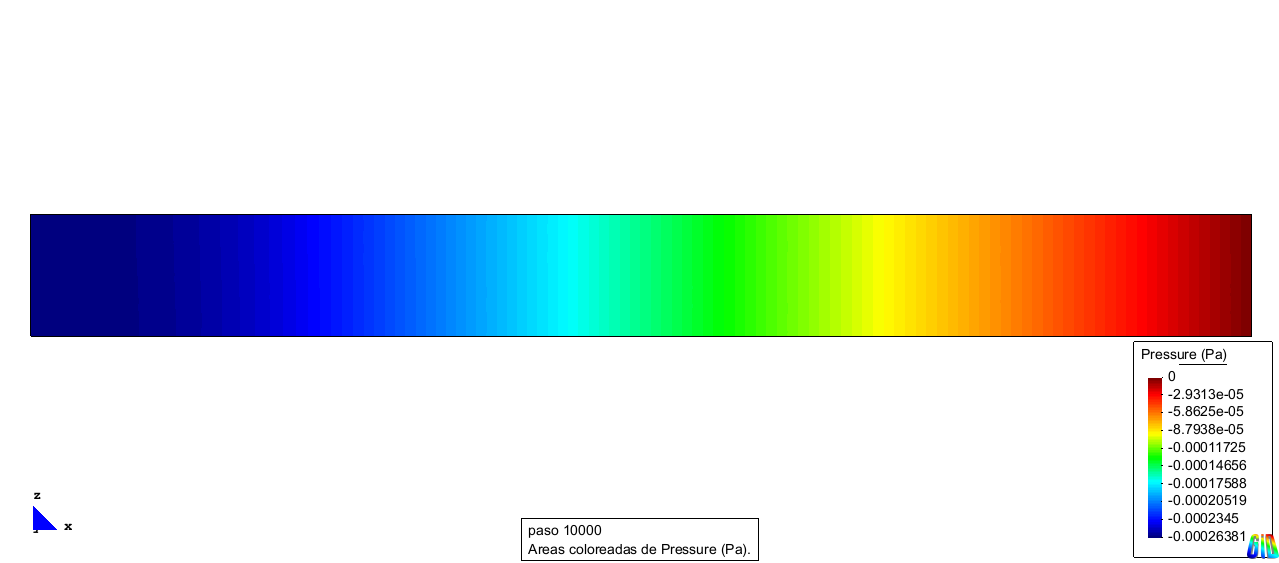
\includegraphics[scale=0.25]{../img/200m/resul/200_XZ_presion_corte_horizontal}}
\caption{Corte en $(x_1,y_1,z_1)=(50,0,0)$ hasta $(x_2,y_2,z_2)=(50,100,0)$ - Vista en el plano XZ - Presión}
\end{figure}
\end{center}
\end{frame}
%
\begin{frame}{Corte transversal - V}
\begin{center}
\begin{figure}[htbp]
\centerline{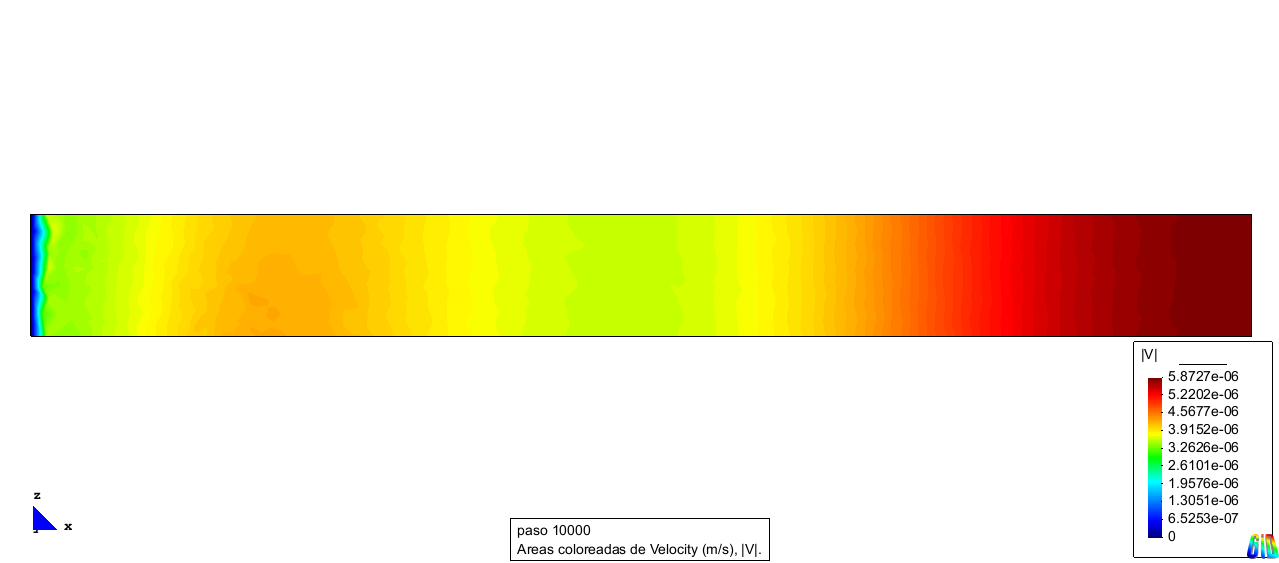
\includegraphics[scale=0.25]{../img/200m/resul/200_XZ_velocidad_corte_horizontal}}
\caption{Corte en $(x_1,y_1,z_1)=(50,0,0)$ hasta $(x_2,y_2,z_2)=(50,100,0)$ - Vista en el plano XZ - Módulo de velocidad}
\end{figure}
\end{center}
\end{frame}
%
\begin{frame}{Gráficas de borde}
\begin{center}
\begin{figure}[htbp]
\centerline{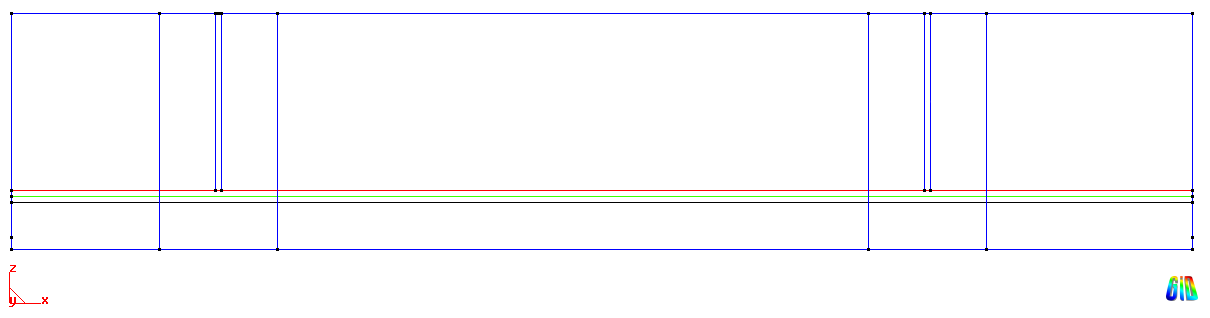
\includegraphics[scale=0.25]{../img/200m/perfiles}}
\end{figure}
\end{center}
\begin{itemize}
\item \color{red} Linea roja: situada sobre la base de los pozos
\item \color{green} Linea verde: situada a $0.5~[m]$ de la base de los pozos
\item \color{black} Linea negra: situada a $1.0~[m]$ de la base de los pozos
\end{itemize}
\end{frame}
%
\begin{frame}{Gráficas de borde situada sobre la base de los pozos}
\begin{center}
\begin{figure}[htbp]
\centerline{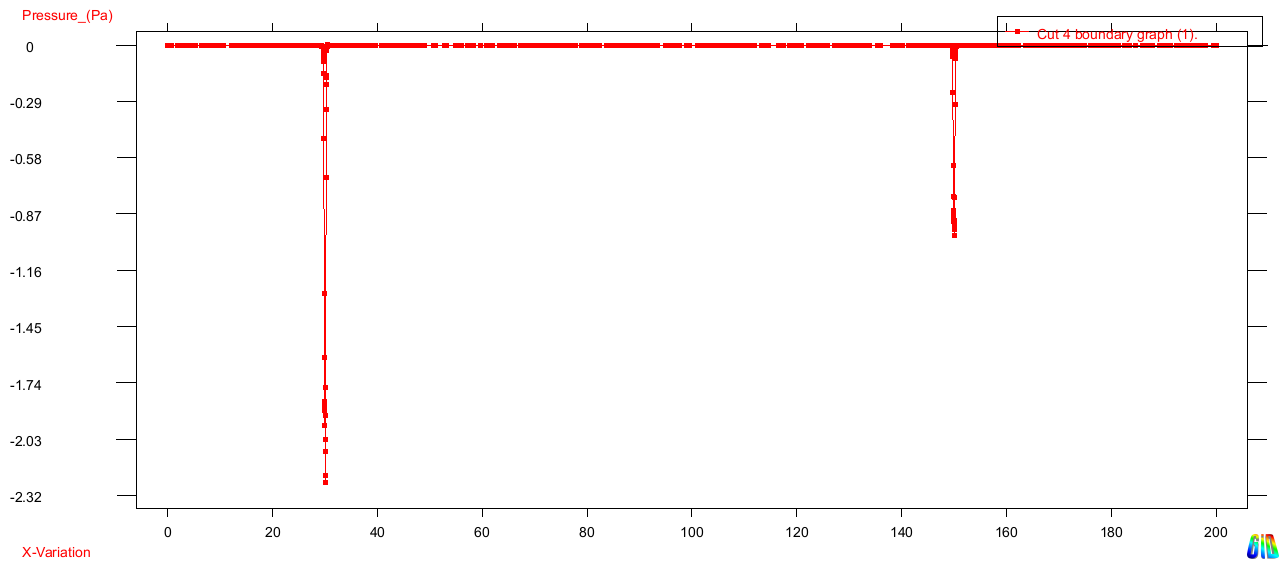
\includegraphics[scale=0.25]{../img/200m/grf/200_grafico_presion_x_centro_pozos_distancia0}}
\caption{Presión}
\end{figure}
\end{center}
\end{frame}
%
%
\begin{frame}{Gráficas de borde situada sobre la base de los pozos}
\begin{center}
\begin{figure}[htbp]
\centerline{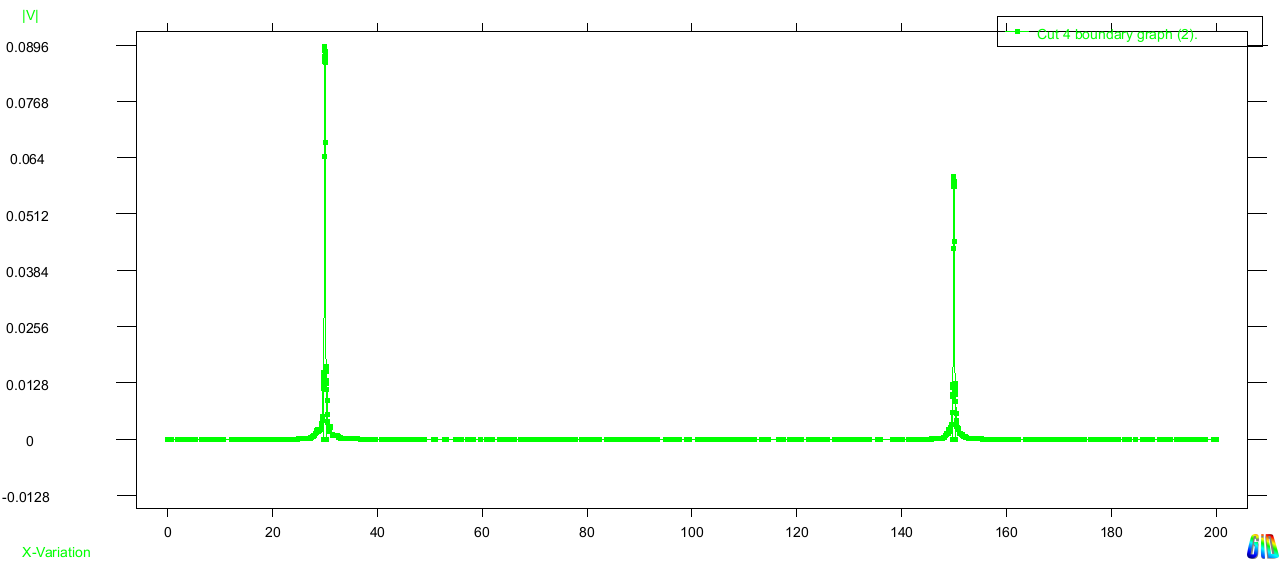
\includegraphics[scale=0.25]{../img/200m/grf/200_grafico_velocidad_x_centro_pozos_distancia0}}
\caption{Velocidad}
\end{figure}
\end{center}
\end{frame}
%
%
\begin{frame}{Gráficas de borde situada a $0.5[m]$ de la base de los pozos}
\begin{center}
\begin{figure}[htbp]
\centerline{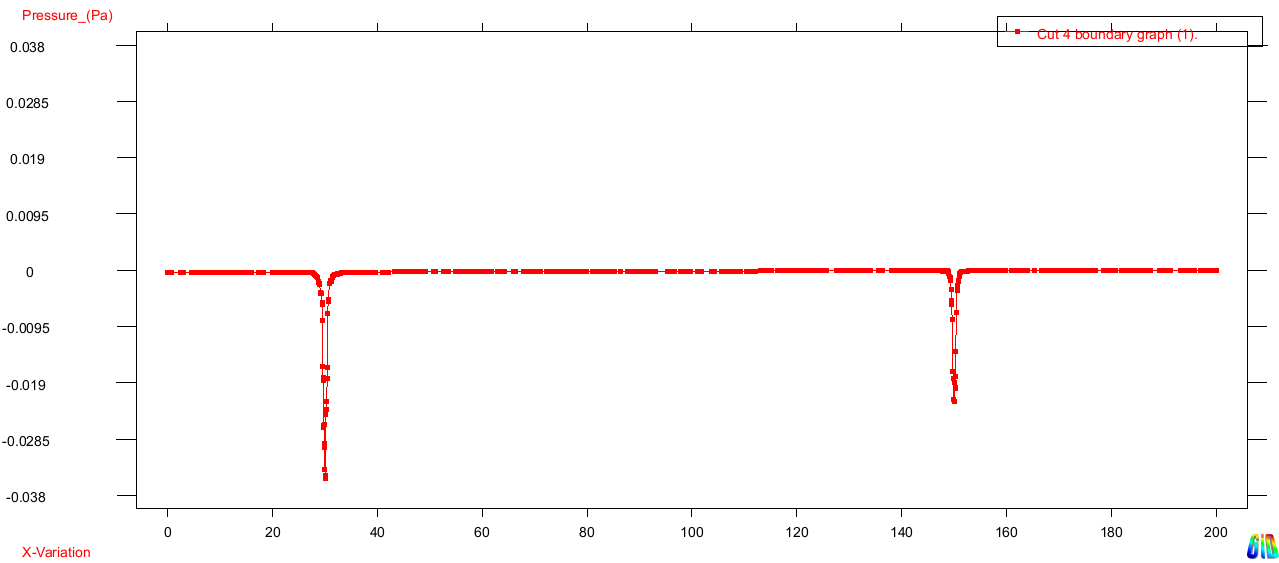
\includegraphics[scale=0.25]{../img/200m/grf/200_grafico_presion_x_centro_pozos_distancia05}}
\caption{Presión}
\end{figure}
\end{center}
\end{frame}
%
%
\begin{frame}{Gráficas de borde situada a $0.5[m]$ de la base de los pozos}
\begin{center}
\begin{figure}[htbp]
\centerline{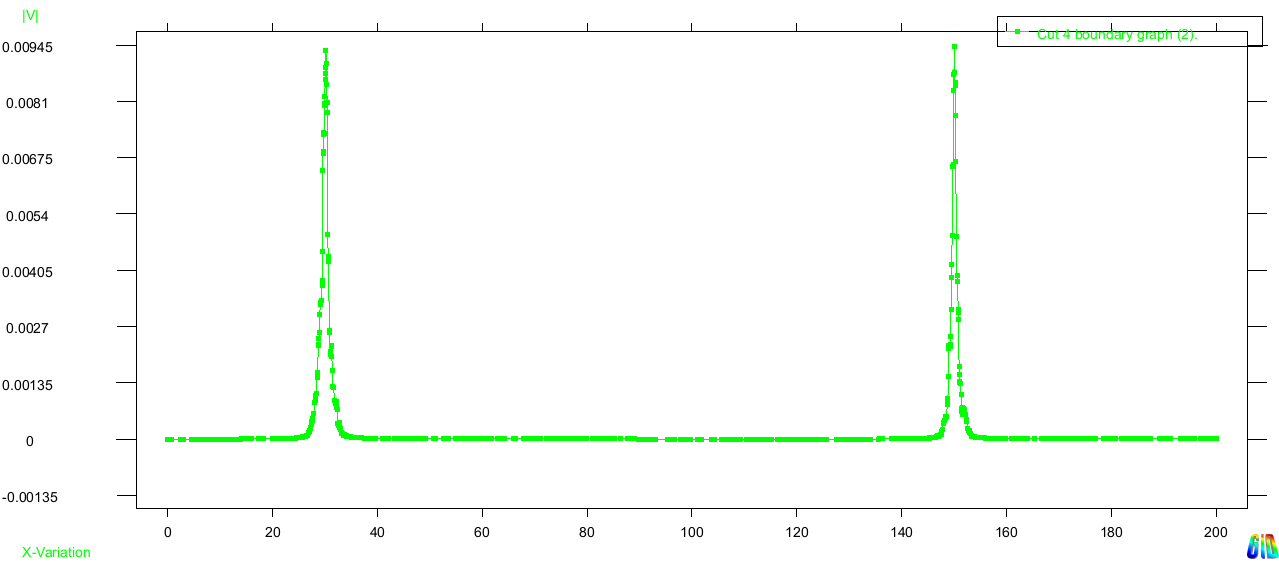
\includegraphics[scale=0.25]{../img/200m/grf/200_grafico_velocidad_x_centro_pozos_distancia05}}
\caption{Velocidad}
\end{figure}
\end{center}
\end{frame}
%
%
\begin{frame}{Gráficas de borde situada a $1.0[m]$ de la base de los pozos}
\begin{center}
\begin{figure}[htbp]
\centerline{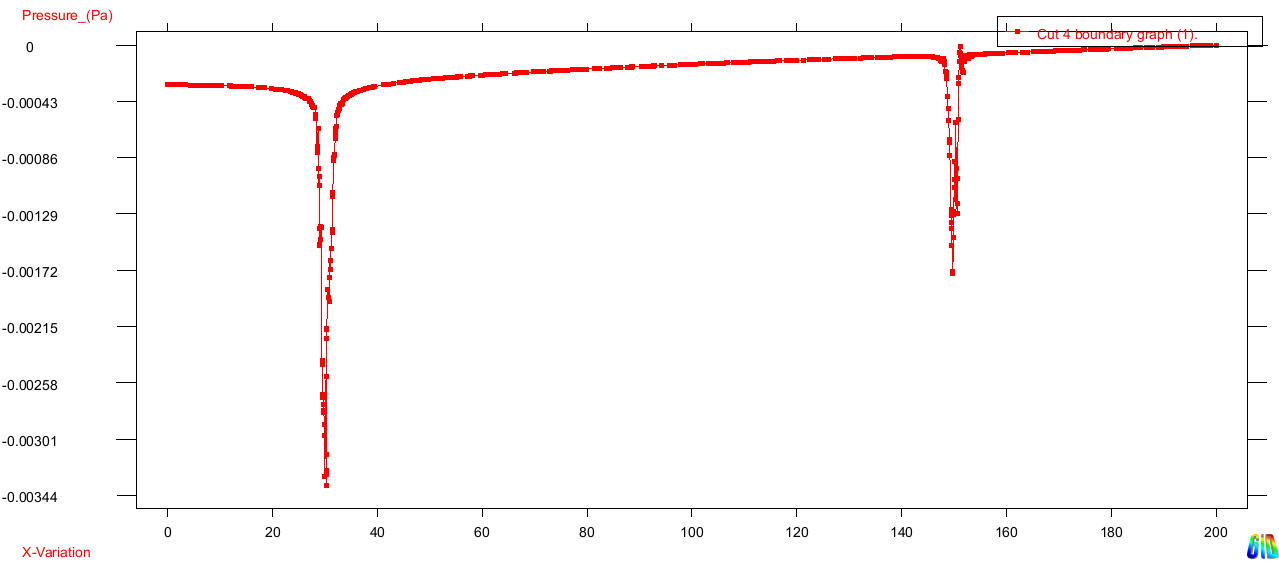
\includegraphics[scale=0.25]{../img/200m/grf/200_grafico_presion_x_centro_pozos_distancia1}}
\caption{Presión}
\end{figure}
\end{center}
\end{frame}
%
%
\begin{frame}{Gráficas de borde situada a $1.0[m]$ de la base de los pozos}
\begin{center}
\begin{figure}[htbp]
\centerline{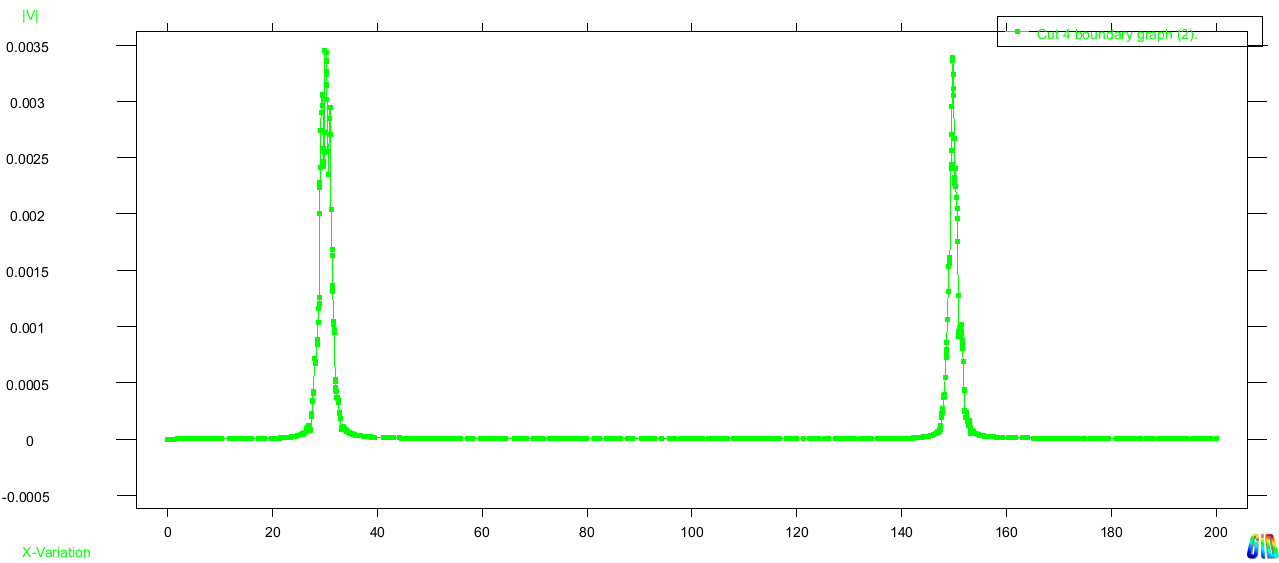
\includegraphics[scale=0.25]{../img/200m/grf/200_grafico_velocidad_x_centro_pozos_distancia1}}
\caption{Velocidad}
\end{figure}
\end{center}
\end{frame}
%
%%%%%%%%%%%%%%%%%%%%%%%%%%%%%%%%%%%%%%%%%%%%%%%%%%%%%%%%%
\section{Conclusiones}
\begin{frame}{Conclusiones}
\begin{itemize}
\item Se integraron los conocimientos incorporados en la materia \emph{``Métodos numéricos y simulación''}.
\item Tener dos geometrías de diferentes dimensiones, permitió comparar resultados.
\item Verificar la interacción (o no) entre las bombas de succión de agua en un acuífero
\begin{itemize}
\item confinado, 
\item homogéneo e 
\item isótropo
\end{itemize}
con un fluido laminar en un  medio poroso.
\item Se supo identificar los datos y condiciones del problema para aplicarlos al software.
\item Se adquirieron conocimientos básicos de Hidrología.
\end{itemize}
\end{frame}
%
%%%%%%%%%%%%%%%%%%%%%%%%%%%%%%%%%%%%%%%%%%%%%%%%%%%%%%%%%
\section{Trabajos futuros}
\begin{frame}{Trabajos futuros}
  \begin{itemize}
  \item Cambiar características del medio poroso - Transmisividad.
  \item Agregado de pozos.
  \item Tamaño del dominio.
  \end{itemize}
\end{frame}
%%%%%%%%%%%%%%%%%%%%%%%%%%%%%%%%%%%%%%%%%%%%%%%%%%%%%%%%%
\section{Bibliografía}
\begin{frame}{Bibliografía}
  \begin{itemize}
  \item ``GID The Personal Pre and Post Processor''. Ayuda de \textbf{GID 9.04}. http://gid.cimne.upc.es/. 13 de septiembre de 2010, 18:00 hs. 
  \item ``Compass Ingeniería y Sistemas''. Ayuda de \textbf{Tdyn3d 5.9.0.11}. http://www.compassis.com/compass. 13 de septiembre de 2010, 18:00 hs.
  \item Apuntes de la materia \textbf{``Métodos numéricos y simulación''}, II-FICH-UNL.
  \item Zienkiewicz,  O.C. y Morgan K. \textbf{Finite Elements and Approximation}. John Wiley \& Sons Australia, Limited. 1983.
  \item Ven Te Chow, David R. Maidment, Larry W. Mays. \textbf{Hidrología aplicada}. McGRAW-HILL. 2000.
 \end{itemize}
\end{frame}
\end{document}